% Two-column preview to approximate published JCIM layout
% Compile: pdflatex preview_twocol && bibtex preview_twocol && pdflatex preview_twocol && pdflatex preview_twocol
%
% This is NOT for submission — use benchmark_paper_jcim.tex (achemso) for that.
% This file previews how the paper will look in the published two-column format.
\documentclass[10pt,twocolumn,letterpaper]{article}

% ===== Page geometry to mimic ACS two-column =====
\usepackage[top=0.75in, bottom=0.75in, left=0.63in, right=0.63in, columnsep=0.25in]{geometry}

% ===== Packages =====
\usepackage{amsmath,amssymb,amsfonts}
\usepackage{graphicx}
\usepackage{booktabs}
\usepackage{subcaption}
\usepackage{siunitx}
\usepackage{adjustbox}
\usepackage{soul}
\usepackage{tikz}
\usetikzlibrary{arrows.meta, positioning, shapes, calc, fit, decorations.pathreplacing}
\usepackage{longtable}
\usepackage{multirow}
\usepackage[dvipsnames]{xcolor}
\usepackage{placeins}
\usepackage[numbers,super,sort&compress]{natbib}
\usepackage[colorlinks,citecolor=blue!60!black,linkcolor=blue!60!black,urlcolor=blue!60!black]{hyperref}
\usepackage{mathptmx}          % Times Roman text + math (ACS house style)
\usepackage[scaled=0.92]{helvet} % Helvetica for sans-serif
\usepackage{courier}            % Courier for monospace
\usepackage[font=small,labelfont=bf]{caption}
\usepackage{titlesec}
\usepackage{float}
\usepackage{enumitem}
\setlist{nosep,leftmargin=*}

% ===== ACS-like section formatting =====
\titleformat{\section}{\normalfont\bfseries\large}{\thesection.}{0.5em}{}
\titleformat{\subsection}{\normalfont\bfseries}{\thesubsection.}{0.5em}{}
\titleformat{\subsubsection}{\normalfont\bfseries\itshape}{\thesubsubsection.}{0.5em}{}
\titlespacing*{\section}{0pt}{1.2ex plus 0.4ex}{0.8ex plus 0.2ex}
\titlespacing*{\subsection}{0pt}{1.0ex plus 0.3ex}{0.6ex plus 0.1ex}

% ===== Custom Commands =====
\newcommand{\vect}[1]{\mathbf{#1}}
\newcommand{\matr}[1]{\mathbf{#1}}

% ===== Reduce float spacing for compact layout =====
\setlength{\textfloatsep}{8pt plus 2pt minus 2pt}
\setlength{\floatsep}{6pt plus 2pt minus 2pt}
\setlength{\intextsep}{6pt plus 2pt minus 2pt}
\setlength{\abovecaptionskip}{4pt}
\setlength{\belowcaptionskip}{2pt}

% ===== Title block =====
\title{\Large\bfseries When Do Simple Models Win? Machine Learning Architectures for UV Absorption Prediction and Insights for General Molecular Property Prediction}

\author{%
Umesh Arampath,$^{a,b,*}$ Bryant Pero,$^{b}$ David Stewart,$^{a}$ and David Demirjian$^{b}$\\[6pt]
{\small\itshape $^{a}$Department of Mathematics, University of Iowa, Iowa City, IA, USA}\\
{\small\itshape $^{b}$Midwest Bioprocessing Center, IL, USA}\\[3pt]
{\small $^{*}$E-mail: uarampath@mwbioprocessing.com}
}

\date{}

\begin{document}

\twocolumn[
  \maketitle
  \begin{@twocolumnfalse}
  \begin{abstract}
\noindent
What determines which machine learning architecture wins for molecular property prediction?
We address this question through a controlled comparison of five models spanning four architecture families: fingerprint-based ensembles (Random Forest, XGBoost), a directed message-passing graph neural network (GNN), a bidirectional gated recurrent network (BiGRU), and a pretrained Transformer, using UV absorption wavelength ($\lambda_{\max}$) prediction as a testbed across 18,755 solute--solvent pairs with stratified 5-fold cross-validation and two external datasets totaling over 40,000 molecules.
The answer depends on the task.
For screening within known chemical space, RF with Morgan fingerprints is optimal: it matches the GNN (RMSE = $31.34 \pm 1.82$ vs.\ $31.69 \pm 3.18$~nm, $p = 0.77$), trains in 15 minutes on a CPU with no hyperparameter tuning, and outperforms all sequence-based models.
For exploring novel scaffolds, deep learning is superior: experimental validation on 16 novel UV-absorbing compounds shows that the GNN (MAE = 26.2~nm), Transformer (26.3~nm), and an optimized BiGRU (28.6~nm; 3-layer, 256-unit architecture identified via Bayesian hyperparameter search) all outperform RF (38.5~nm), as learned representations generalize where fixed fingerprints cannot.
In either case, encoding solvent identity improves all models: a simple SMILES/fingerprint concatenation strategy yields 6--8\% RMSE reductions across fingerprint, graph, and recurrent architectures ($p < 0.02$), without domain-specific descriptor engineering.
Interpretability analysis confirms that both RF feature importance and BiGRU gradient saliency independently highlight the same chromophore motifs, and that architectures with local inductive bias systematically outperform global-attention Transformers on this locally determined property.
  \end{abstract}
  \vspace{0.8em}
  \noindent\textbf{Keywords:} UV absorption $\cdot$ molecular property prediction $\cdot$ deep learning $\cdot$ random forest $\cdot$ Morgan fingerprints $\cdot$ graph neural network $\cdot$ Chemprop $\cdot$ ChemBERTa $\cdot$ solvent effects
  \vspace{1.2em}
  \end{@twocolumnfalse}
]

% ===== Introduction =====
\section{Introduction}
\label{sec:introduction}

Ultraviolet--visible (UV--Vis) absorption spectroscopy is a fundamental technique in chemistry, with the wavelength of maximum absorption ($\lambda_{\max}$) serving as a key property for molecular characterization, photosafety assessment, and materials design.\cite{flemingMolecular2010}
When a molecule absorbs UV--Vis light, electrons undergo transitions between molecular orbitals; $\lambda_{\max}$ corresponds to the most probable electronic transition and is governed by the extent of $\pi$-conjugation, heteroatom substituents, and molecular geometry.\cite{reichardt2011solvents}
Experimental determination of $\lambda_{\max}$ requires synthesizing and measuring each compound, creating a demand for accurate \textit{in silico} prediction methods that can accelerate screening of large chemical libraries.\cite{ghosh2019deep}

Machine learning (ML) approaches for molecular property prediction have proliferated in recent years, spanning classical methods using engineered molecular descriptors (e.g., Morgan fingerprints\cite{rogers2010extended} with Random Forest\cite{breiman2001random}) to deep learning architectures that learn representations directly from molecular strings (SMILES\cite{weininger1988smiles}) or graphs.\cite{gilmer2017neural}
Large curated datasets such as the Joung+Beard database\cite{joung2020experimental, beard2019comparative} and benchmarking suites like MoleculeNet\cite{wuMoleculeNet2018} have accelerated progress, yet systematic comparisons across multiple datasets with consistent methodology remain rare. Without such comparisons, practitioners lack guidance on which model families to deploy for a given chemistry domain.
Recent work has highlighted that well-tuned classical models can match or exceed complex deep learning architectures for molecular property prediction,\cite{panapitiya2022evaluation, walters2021applications} suggesting that no universal ``best model'' exists; rather, the optimal choice depends on the interplay between molecular representation, property type, and the novelty of target compounds relative to training data.

The UV absorption prediction task presents several distinctive challenges that make it an ideal benchmarking target:
\begin{enumerate}
    \item \textbf{Solvent dependence:} $\lambda_{\max}$ varies with solvent environment (solvatochromism), requiring models to encode both solute structure and solvent identity.
    \item \textbf{Representation diversity:} Although absorption depends on electronic structure influenced by molecular geometry, our results show that 1D representations (fingerprints, SMILES) capture the dominant structure--property relationships for UV absorption, with 3D methods offering advantages primarily for structurally diverse datasets.
    \item \textbf{Diverse benchmarks:} Multiple published datasets with varying sizes, chemical spaces, and evaluation protocols enable comprehensive assessment.
    \item \textbf{Practical relevance:} ICH~S10 guidelines require photosafety screening of pharmaceutical compounds, where $\lambda_{\max}$ prediction serves as a first-pass filter.
\end{enumerate}

In this work, we present a benchmark study comparing five ML approaches---Random Forest, XGBoost, Chemprop (D-MPNN), Bidirectional GRU, and ChemBERTa---spanning fingerprint, graph, recurrent, and Transformer architectures for $\lambda_{\max}$ prediction.
Our key contributions are:
\begin{itemize}
    \item \textbf{Practical model selection guidance:} RF is optimal for in-distribution screening (fast, no GPU, no tuning needed); deep learning models generalize better to novel compounds. We validate this on 16 experimentally measured UV-absorbing molecules.
    \item \textbf{Controlled multi-architecture comparison} across three datasets using published evaluation protocols. Chemprop (D-MPNN) with default hyperparameters sets new state-of-the-art results on both external datasets, while RF and Chemprop are statistically tied on primary cross-validation.
    \item \textbf{Optimized BiGRU architecture} via Bayesian hyperparameter search (3-layer, 256-unit, 4.8\% RMSE improvement), demonstrating that a sequence-based approach operating on raw SMILES can match graph and fingerprint methods without compromising prediction accuracy.
    \item \textbf{Architecture-independent solvent encoding:} a simple concatenation strategy yields 6--8\% RMSE reductions across fingerprint, graph, and recurrent models ($p < 0.02$), without domain-specific descriptor engineering.
    \item \textbf{Locality-of-property hypothesis:} architectures with local inductive bias systematically outperform global-attention Transformers on UV absorption. All three encode molecular structure with an implicit spatial cutoff (Morgan fingerprints through a fixed radius, D-MPNN through bounded message-passing depth, and BiGRU through gradient decay in the recurrent hidden state), while Transformers impose no such locality constraint through global self-attention.
    \item \textbf{Photosafety application:} ICH~S10 classification on a reconstructed Reaxys dataset validates practical utility.
\end{itemize}

The choice of molecular representation fundamentally determines which ML methods can be applied.
SMILES (Simplified Molecular Input Line Entry System)\cite{weininger1988smiles} encodes molecular graphs as character strings, enabling NLP-inspired sequence models (RNNs, Transformers), while Morgan circular fingerprints\cite{rogers2010extended} encode local chemical environments as fixed-length binary vectors amenable to classical tree-based ensembles.\cite{landrum2016rdkit, wuMoleculeNet2018}
Our benchmark compares three representation families: fingerprint-based models (RF, XGBoost), a graph neural network (Chemprop D-MPNN), and sequence-based models (BiGRU, ChemBERTa) on the same prediction task.
Figure~\ref{fig:benchmark_framework} provides an overview of this multi-pathway framework.

% ===== Figure 1: Benchmark Framework (wide) =====
\begin{figure*}[!ht]
    \centering
    % ===== (a) Input and Representation =====
    \begin{subfigure}[b]{\textwidth}
    \centering
    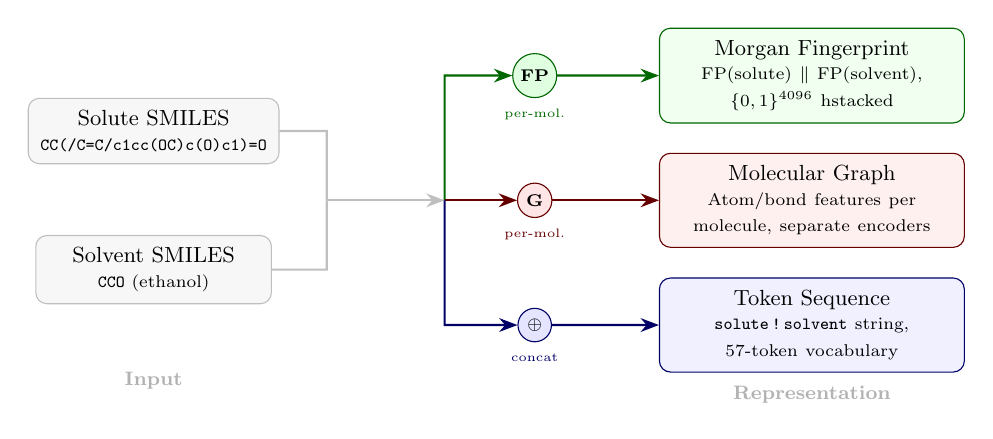
\begin{tikzpicture}[scale=0.88, every node/.style={scale=0.88},
        >=Stealth,
        box/.style={draw, rounded corners=4pt, align=center, font=\small, inner sep=5pt},
        arr/.style={->, thick, draw=gray!50},
    ]
    \node[box, fill=gray!6, draw=gray!50, minimum width=3.4cm] (mol) at (0, 1.0)
        {Solute SMILES\\[-1pt]{\scriptsize\texttt{CC(/C=C/c1cc(OC)c(O)c1)=O}}};
    \node[box, fill=gray!6, draw=gray!50, minimum width=3.4cm] (solv) at (0, -1.0)
        {Solvent SMILES\\[-1pt]{\scriptsize\texttt{CCO} (ethanol)}};
    \draw[thick, draw=gray!50] (mol.east) -- (2.5, 1.0) -- (2.5, 0);
    \draw[thick, draw=gray!50] (solv.east) -- (2.5, -1.0) -- (2.5, 0);
    \coordinate (fork) at (4.2, 0);
    \draw[arr] (2.5, 0) -- (fork);
    % Green path
    \node[draw, circle, fill=green!12, draw=green!40!black, inner sep=2pt, font=\scriptsize\bfseries] (fpnode) at (5.5, 1.8) {FP};
    \node[font=\tiny, green!40!black, below=1pt of fpnode] {per-mol.};
    \node[box, fill=green!6, draw=green!40!black, minimum width=4.4cm, text width=4.0cm] (fp) at (9.5, 1.8)
        {Morgan Fingerprint\\[-1pt]{\scriptsize FP(solute) $\|$ FP(solvent), $\{0,1\}^{4096}$ hstacked}};
    \draw[arr, draw=green!40!black] (fork) -- (4.2, 1.8) -- (fpnode);
    \draw[arr, draw=green!40!black] (fpnode) -- (fp.west);
    % Red path
    \node[draw, circle, fill=red!10, draw=red!40!black, inner sep=2pt, font=\scriptsize\bfseries] (graphnode) at (5.5, 0) {G};
    \node[font=\tiny, red!40!black, below=1pt of graphnode] {per-mol.};
    \node[box, fill=red!6, draw=red!40!black, minimum width=4.4cm, text width=4.0cm] (mg) at (9.5, 0)
        {Molecular Graph\\[-1pt]{\scriptsize Atom/bond features per molecule, separate encoders}};
    \draw[arr, draw=red!40!black] (fork) -- (4.2, 0) -- (graphnode);
    \draw[arr, draw=red!40!black] (graphnode) -- (mg.west);
    % Blue path
    \node[draw, circle, fill=blue!10, draw=blue!40!black, inner sep=2pt, font=\scriptsize\bfseries] (cat) at (5.5, -1.8) {$\oplus$};
    \node[font=\tiny, blue!40!black, below=1pt of cat] {concat};
    \node[box, fill=blue!6, draw=blue!40!black, minimum width=4.4cm, text width=4.0cm] (seq) at (9.5, -1.8)
        {Token Sequence\\[-1pt]{\scriptsize \texttt{solute\,!\,solvent} string, 57-token vocabulary}};
    \draw[arr, draw=blue!40!black] (fork) -- (4.2, -1.8) -- (cat);
    \draw[arr, draw=blue!40!black] (cat) -- (seq.west);
    \node[font=\footnotesize\bfseries, gray!60] at (0, -2.6) {\textsc{Input}};
    \node[font=\footnotesize\bfseries, gray!60] at (9.5, -2.8) {\textsc{Representation}};
    \end{tikzpicture}
    \caption{Input and representation. Both solute and solvent SMILES feed three pathways.}
    \label{fig:framework_input}
    \end{subfigure}

    \vspace{0.3cm}

    % ===== (b) Models and Prediction =====
    \begin{subfigure}[b]{\textwidth}
    \centering
    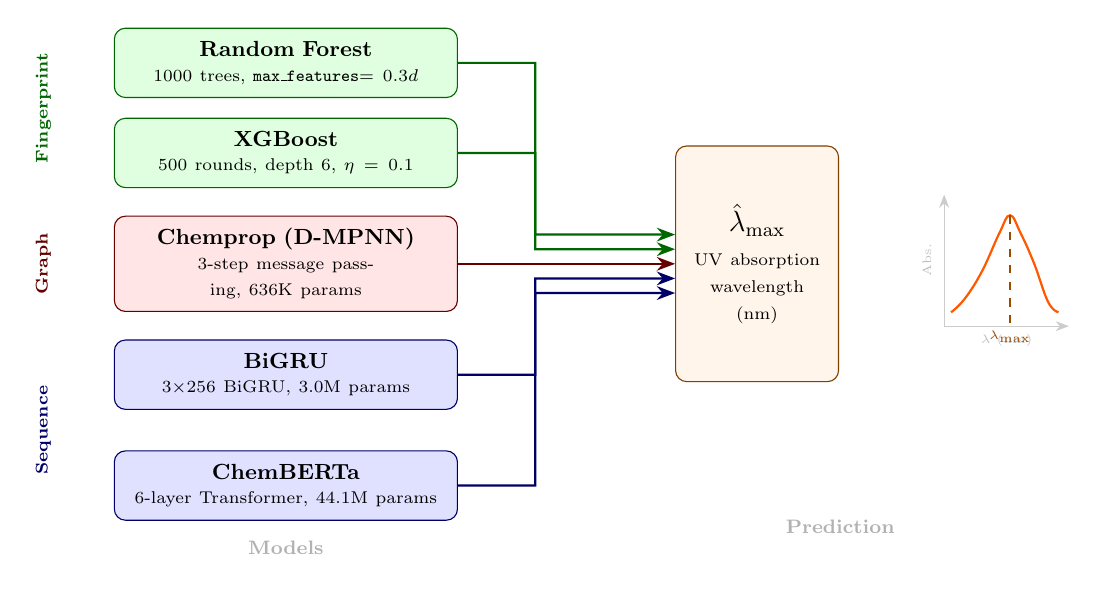
\begin{tikzpicture}[scale=0.88, every node/.style={scale=0.88},
        >=Stealth,
        box/.style={draw, rounded corners=4pt, align=center, font=\small,
                     inner sep=5pt, text width=4.6cm, minimum height=1.0cm},
        arr/.style={->, thick},
    ]
    \node[box, fill=green!12, draw=green!40!black] (rf) at (0, 2.9)
        {\textbf{Random Forest}\\[-1pt]{\scriptsize 1000 trees, \texttt{max\_features}$= 0.3d$}};
    \node[box, fill=green!12, draw=green!40!black] (xgb) at (0, 1.6)
        {\textbf{XGBoost}\\[-1pt]{\scriptsize 500 rounds, depth 6, $\eta = 0.1$}};
    \node[box, fill=red!10, draw=red!40!black] (chemprop) at (0, 0)
        {\textbf{Chemprop (D-MPNN)}\\[-1pt]{\scriptsize 3-step message passing, 636K params}};
    \node[box, fill=blue!12, draw=blue!40!black] (bigru) at (0, -1.6)
        {\textbf{BiGRU}\\[-1pt]{\scriptsize 3$\times$256 BiGRU, 3.0M params}};
    \node[box, fill=blue!12, draw=blue!40!black] (cb) at (0, -3.2)
        {\textbf{ChemBERTa}\\[-1pt]{\scriptsize 6-layer Transformer, 44.1M params}};
    \node[font=\scriptsize\bfseries, green!40!black, rotate=90, anchor=center] at (-3.5, 2.25) {Fingerprint};
    \node[font=\scriptsize\bfseries, red!40!black, rotate=90, anchor=center] at (-3.5, 0) {Graph};
    \node[font=\scriptsize\bfseries, blue!40!black, rotate=90, anchor=center] at (-3.5, -2.4) {Sequence};
    \node[box, fill=orange!8, draw=orange!50!black, text width=2.0cm,
          minimum height=3.4cm] (out) at (6.8, 0)
        {\textbf{\large $\hat{\lambda}_{\max}$}\\[3pt]{\scriptsize UV absorption}\\{\scriptsize wavelength (nm)}};
    \draw[arr, draw=green!40!black] (rf.east)       -- (3.6, 2.9)   |- ([yshift=12pt]out.west);
    \draw[arr, draw=green!40!black] (xgb.east)      -- (3.6, 1.6)   |- ([yshift=6pt]out.west);
    \draw[arr, draw=red!40!black]   (chemprop.east) -- (3.6, 0)     |- (out.west);
    \draw[arr, draw=blue!40!black]  (bigru.east)    -- (3.6, -1.6)  |- ([yshift=-6pt]out.west);
    \draw[arr, draw=blue!40!black]  (cb.east)       -- (3.6, -3.2)  |- ([yshift=-12pt]out.west);
    \begin{scope}[shift={(9.5, 0)}]
        \draw[gray!40, ->] (0,-0.9) -- (0,1.0);
        \node[font=\tiny, gray!50, rotate=90] at (-0.25, 0.05) {Abs.};
        \draw[gray!40, ->] (0,-0.9) -- (1.8,-0.9);
        \node[font=\tiny, gray!50] at (0.9, -1.1) {$\lambda$ (nm)};
        \draw[orange!70!red, thick, smooth, tension=0.7]
            plot coordinates {(0.1,-0.7) (0.3,-0.5) (0.55,-0.1) (0.8,0.45) (0.95,0.7) (1.1,0.45) (1.3,0.0) (1.5,-0.55) (1.65,-0.7)};
        \draw[dashed, orange!60!black] (0.95,0.7) -- (0.95,-0.9);
        \node[font=\tiny\bfseries, orange!60!black] at (0.95, -1.05) {$\lambda_{\max}$};
    \end{scope}
    \node[font=\footnotesize\bfseries, gray!60] at (0, -4.1) {\textsc{Models}};
    \node[font=\footnotesize\bfseries, gray!60] at (8.0, -3.8) {\textsc{Prediction}};
    \end{tikzpicture}
    \caption{Models and prediction. All five models predict $\lambda_{\max}$.}
    \label{fig:framework_models}
    \end{subfigure}

    \caption{Benchmark framework for UV absorption prediction. (a)~Three representation pathways: Morgan fingerprints (green), molecular graphs (red), and token sequences (blue). (b)~Five models spanning fingerprint, graph, and sequence architectures.}
    \label{fig:benchmark_framework}
\end{figure*}


\FloatBarrier
% ===== Related Work =====
\section{Related Work}
\label{sec:related_work}

Machine learning for UV absorption prediction has evolved from classical QSAR models using handcrafted descriptors to modern deep learning approaches operating on molecular graphs and strings.

\textbf{Fingerprint-based methods.}
Morgan circular fingerprints,\cite{rogers2010extended} also known as extended-connectivity fingerprints (ECFP), encode local atomic environments as fixed-length binary vectors and have become the de facto standard molecular representation for classical ML.\cite{wuMoleculeNet2018}
When combined with tree-based ensemble methods such as Random Forests\cite{breiman2001random} or gradient boosting,\cite{chen2016xgboost} fingerprint-based models achieve competitive performance on many molecular property prediction tasks, including aqueous solubility,\cite{delaney2004esol, panapitiya2022evaluation} toxicity,\cite{mayr2016deeptox} and UV absorption.\cite{mamede2021machine}
Mamede et al.\cite{mamede2021machine} used RF with Morgan fingerprints for ICH~S10\cite{ICH2013S10} photosafety classification on a 74,784-compound Reaxys dataset, achieving sensitivity 0.90 and specificity 0.88.

\textbf{Sequence models on SMILES.}
The SMILES representation\cite{weininger1988smiles} maps molecular graphs to character strings, enabling natural language processing techniques for molecular property prediction.
Recurrent neural networks,\cite{elman1990finding} including Long Short-Term Memory (LSTM)\cite{hochreiter1997long} and Gated Recurrent Unit (GRU)\cite{cho2014learning} architectures, process SMILES as sequential data, learning molecular features without explicit descriptor engineering.
Bidirectional variants (BiGRU, BiLSTM)\cite{schuster1997bidirectional} capture context from both directions, improving representation quality for molecular strings.
Liu et al.\ combined BiGRU with GraphSAGE for molecular toxicity prediction on Tox21;\cite{liuPredictionMolecularToxicity2023} we adopt only their BiGRU component for SMILES-based regression.
More recently, Transformer architectures\cite{vaswani2017attention} have been applied to SMILES-based property prediction.
Chen et al.\cite{chenMolecularLanguage2023} systematically compared RNNs and Transformers for molecular language modeling, finding that RNNs better capture local structural features while Transformers excel at global properties and longer sequences.
Jiang et al.\cite{jiang2023trangru} further validated this local/global distinction in their TranGRU architecture.

\textbf{Graph neural networks.}
GNNs operate directly on molecular graphs through iterative message passing,\cite{gilmer2017neural} learning atom-level representations from connectivity and atomic features.
Joung et al.\cite{joung2021deep} reported a GCNN achieving RMSE = 26.6~nm on their Deep4Chem database.
Jung et al.\cite{jung2024machine} compared multiple architectures including a GBFS pipeline achieving RMSE = 32.2~nm.

\textbf{Solvent effects.}
Solvatochromism, the shift in absorption wavelength as a function of solvent environment, is a well-studied phenomenon.\cite{reichardt2011solvents}
Despite its importance, most ML studies for UV absorption either ignore solvent effects entirely or use categorical solvent labels.

\textbf{Benchmarking perspective.}
The MoleculeNet benchmark suite\cite{wuMoleculeNet2018} established a standardized framework for comparing molecular ML models, but UV absorption is not among its benchmarks.
Recent work has highlighted that well-tuned classical models often match or exceed complex architectures,\cite{panapitiya2022evaluation, walters2021applications} challenging the assumption that deep learning always outperforms simpler methods.


% ===== Methods =====
\section{Methods}
\label{sec:methods}

\subsection{Dataset Description and Preparation}
\label{sec:dataset}

Our primary dataset combines the Joung et al.\ Experimental Database of Optical Properties\cite{joung2020experimental} and the Beard et al.\ Comparative Dataset.\cite{beard2019comparative}
Data curation proceeded as follows: (1)~SMILES strings were canonicalized using RDKit;\cite{landrumRdkitRdkit2020_03_12020} (2)~entries with invalid SMILES were removed; (3)~duplicates were identified by matching canonical SMILES and solvent identity; (4)~solvent names were standardized and mapped to canonical SMILES.
After merging, deduplication, and canonicalization, the combined dataset contains \textbf{18,755 solute--solvent pairs} spanning 7,016 unique chromophores and 365 solvents.
Target values range from 200 to 900~nm, with a median of 325~nm.

\begin{table}[htbp]
\centering
\caption{Summary of the primary Joung+Beard dataset.}
\label{tab:dataset_summary}
\small
\begin{tabular}{lr}
\toprule
\textbf{Attribute} & \textbf{Value} \\
\midrule
Total records & 18,755 \\
Unique chromophores & 7,016 \\
Unique solvents & 365 \\
$\lambda_{\max}$ range & 200--900 nm \\
$\lambda_{\max}$ median & 325 nm \\
SMILES vocabulary size & 57 tokens \\
Max sequence length & 650 tokens \\
\bottomrule
\end{tabular}
\end{table}


\subsection{Evaluation Protocol}
\label{sec:evaluation}

For the primary dataset, we use \textbf{stratified 5-fold cross-validation}\cite{kohavi1995study} with a 64/16/20 train/validation/test split.
Stratification is performed on solvent identity to ensure representative solvent coverage in each fold.
For deep learning models, the validation set is used exclusively for early stopping (patience = 25 epochs), preventing data leakage from the test set.
For fingerprint-based models, training uses only the training fold.

Metrics are reported as mean $\pm$ standard deviation across five folds: root-mean-square error (RMSE), mean absolute error (MAE), coefficient of determination ($R^2$), and Pearson correlation coefficient ($r$).
Statistical significance is assessed using paired $t$-tests across fold RMSE values ($\alpha = 0.05$).

For external datasets, we use the exact split protocols published by the original authors.


\subsection{Random Forest with Morgan Fingerprints}
\label{sec:rf}

Random Forest (RF)\cite{breiman2001random} is an ensemble method that constructs $B$ decision trees, each trained on a bootstrap sample, and averages their predictions:
\begin{equation}
    \hat{y}(\vect{x}) = \frac{1}{B} \sum_{b=1}^{B} T_b(\vect{x})
\end{equation}
The input representation is the Morgan circular fingerprint\cite{rogers2010extended} ($r=2$, $n=2048$ bits).
For solvent-aware models, solute and solvent fingerprints are concatenated (4096 bits total).
Hyperparameters were selected via grid search over 432 configurations; the optimal uses $B = 1000$ trees, no maximum depth constraint, and $\lfloor 0.3d \rfloor$ features per split.


\subsection{Gradient Boosting (XGBoost)}
\label{sec:xgboost}

XGBoost\cite{chen2016xgboost} constructs an additive ensemble of decision trees trained sequentially:
\begin{equation}
    \hat{y}(\vect{x}) = \sum_{t=1}^{T} \eta \cdot f_t(\vect{x})
\end{equation}
We use $T = 500$ rounds, max depth 6, $\eta = 0.1$, and histogram-based tree construction with the same fingerprint input.


\subsection{Chemprop (D-MPNN)}
\label{sec:chemprop}

Chemprop\cite{yangAnalyzingLearnedMolecular2019} implements a Directed Message Passing Neural Network that operates on molecular graphs by passing messages along directed bonds:
\begin{equation}
    \vect{h}_{vw}^{(t)} = \tau\!\left(\vect{h}_{vw}^{(0)} + \matr{W}_t \sum_{u \in N(v) \setminus w} \vect{h}_{uv}^{(t-1)}\right)
\end{equation}
We use the multicomponent variant with separate D-MPNN encoders for solute and solvent ($d_h = 300$), 3 message-passing steps, mean aggregation, and default hyperparameters (636K total parameters).
Training uses the Noam learning rate schedule (warmup $10^{-4}$ to $10^{-3}$, then decay to $10^{-4}$), batch size 64, and early stopping (patience 15).


\subsection{Bidirectional GRU (BiGRU)}
\label{sec:bigru}

The GRU\cite{cho2014learning} addresses vanishing gradients through update and reset gates:
\begin{align}
    \vect{z}_t &= \sigma(\matr{W}_z \vect{x}_t + \matr{U}_z \vect{h}_{t-1} + \vect{b}_z) \\
    \vect{r}_t &= \sigma(\matr{W}_r \vect{x}_t + \matr{U}_r \vect{h}_{t-1} + \vect{b}_r) \\
    \vect{h}_t &= (1 - \vect{z}_t) \odot \vect{h}_{t-1} + \vect{z}_t \odot \tilde{\vect{h}}_t
\end{align}

Our BiGRU processes character-level tokenized SMILES (57-token vocabulary).
The default architecture uses 2 stacked BiGRU layers (128 units per direction, $\sim$470K parameters).
After Bayesian HPO (25 Optuna trials\cite{akiba2019optuna}), the optimized architecture uses 3 layers with 256 units ($\sim$3.0M parameters), achieving RMSE = $34.71 \pm 1.40$~nm (4.8\% improvement).


\subsection{ChemBERTa (Transformer)}
\label{sec:chemberta}

ChemBERTa\cite{chithrananda2020chemberta} is a RoBERTa-based\cite{liu2019roberta} Transformer pretrained on SMILES from the ZINC database.
The model has 6 Transformer layers, 12 attention heads, hidden dimension 768, and 44.1M parameters.
We fine-tune all layers with AdamW ($\text{lr} = 5 \times 10^{-5}$), Huber loss ($\beta = 10$), batch size 32, and early stopping (patience 15).


\subsection{Solvent Information Encoding}
\label{sec:solvent}

We encode solvent information by concatenating solute and solvent SMILES:
\begin{equation}
    S_{\text{input}} = \texttt{!} \oplus S_{\text{solute}} \oplus \texttt{!} \oplus S_{\text{solvent}} \oplus \texttt{E}
\end{equation}
For fingerprint models, Morgan FPs are computed separately and concatenated (2048 + 2048 = 4096 dimensions).
For Chemprop, separate D-MPNN encoders process solute and solvent graphs.


\subsection{External Datasets}
\label{sec:datasets}

\textbf{Deep4Chem} (Joung 2020):\cite{joung2021deep} 30,094 chromophore--solvent combinations; after deduplication, 17,683 records. Published GCNN baseline: RMSE = 26.6~nm. Split: 80/10/10 random.

\textbf{Jung et al.\ (2024)}:\cite{jung2024machine} $\sim$26,000 records. Published baselines: GBFS RMSE = 32.2~nm, Multifidelity RMSE = 31.3~nm. Split: 72/18/10 random.


% ===== Results =====
\section{Results and Discussion}
\label{sec:results}

\subsection{Model Comparison on Joung+Beard Dataset}
\label{sec:model_comparison}

Table~\ref{tab:model_comparison} presents the primary cross-validated results.

\begin{table}[htbp]
\centering
\caption{Model comparison on the Joung+Beard dataset (18,755 samples, stratified 5-fold CV, 64/16/20 split). Best in bold. $\pm$ = std across folds.}
\label{tab:model_comparison}
\small
\begin{tabular}{lcccc}
\toprule
\textbf{Model} & \textbf{RMSE} & \textbf{MAE} & $\boldsymbol{R^2}$ & $\boldsymbol{r}$ \\
\midrule
RF + Morgan FP        & \textbf{31.34} & \textbf{15.16} & \textbf{0.914} & \textbf{0.956} \\
                      & $\pm$1.82      & $\pm$0.44      & $\pm$0.010     & $\pm$0.005     \\[2pt]
Chemprop (D-MPNN)     & 31.69          & 16.84          & 0.911          & 0.955          \\
                      & $\pm$3.18      & $\pm$1.74      & $\pm$0.016     & $\pm$0.009     \\[2pt]
XGBoost + Morgan FP   & 33.70          & 20.05          & 0.900          & 0.950          \\
                      & $\pm$1.61      & $\pm$0.48      & $\pm$0.009     & $\pm$0.005     \\[2pt]
BiGRU (tuned)         & 34.71          & 18.09          & 0.894          & 0.946          \\
                      & $\pm$1.40      & $\pm$0.59      & $\pm$0.009     & $\pm$0.005     \\[2pt]
BiGRU (default)       & 36.45          & 20.70          & 0.884          & 0.940          \\
                      & $\pm$1.12      & $\pm$0.51      & $\pm$0.006     & $\pm$0.003     \\[2pt]
ChemBERTa             & 50.39          & 24.31          & 0.777          & 0.899          \\
                      & $\pm$2.30      & $\pm$1.04      & $\pm$0.019     & $\pm$0.009     \\
\bottomrule
\end{tabular}
\end{table}

RF achieves the best mean RMSE (31.34~nm), closely followed by Chemprop (31.69~nm); the difference is not statistically significant ($p = 0.77$, paired $t$-test).
Both outperform BiGRU (tuned: 34.71~nm) and ChemBERTa (50.39~nm).
The strong performance of local-feature models is consistent with the physics of UV absorption: $\lambda_{\max}$ is determined by local chromophore features (conjugation, substituents), and both RF (radius-2 fingerprints) and Chemprop (3-hop message passing) encode these local neighborhoods.\cite{flemingMolecular2010}


\subsection{Effect of Solvent Information}
\label{sec:solvent_ablation}

\begin{table}[htbp]
\centering
\caption{Solvent ablation: effect of encoding solvent identity.}
\label{tab:solvent_ablation}
\small
\begin{tabular}{lcc}
\toprule
\textbf{Model} & \textbf{RMSE +Solv.} & \textbf{RMSE Solute only} \\
\midrule
RF       & 31.34 $\pm$ 1.82 & 34.13 $\pm$ 1.44 \\
Chemprop & 31.69 $\pm$ 3.18 & 33.78 $\pm$ 2.73 \\
BiGRU    & 36.45 $\pm$ 1.12 & 39.03 $\pm$ 1.37 \\
\bottomrule
\end{tabular}
\end{table}

Solvent encoding reduces RF RMSE by 8\% ($p = 0.0003$), Chemprop by 6\% ($p = 0.012$), and BiGRU by 7\% ($p = 0.018$), confirming effectiveness across all architectures.


\subsection{Cross-Dataset Benchmarking}
\label{sec:cross_dataset}

\begin{table}[htbp]
\centering
\caption{Cross-dataset benchmarking. $\dagger$Published results. Best of our models in bold.}
\label{tab:cross_dataset}
\small
\begin{tabular}{llcc}
\toprule
\textbf{Dataset} & \textbf{Model} & \textbf{RMSE} & $\boldsymbol{R^2}$ \\
\midrule
\multirow{5}{*}{\shortstack[l]{Deep4Chem\\(80/10/10)}}
  & GCNN$^\dagger$   & 26.6           & ---   \\
  & Our Chemprop     & \textbf{19.13} & \textbf{0.967} \\
  & Our RF           & 22.70          & 0.954 \\
  & Our BiGRU        & 27.07          & 0.934 \\
  & Our ChemBERTa    & 35.90          & 0.884 \\
\midrule
\multirow{5}{*}{\shortstack[l]{Jung 2024\\(72/18/10)}}
  & GBFS$^\dagger$   & 32.2           & 0.91  \\
  & MF$^\dagger$     & 31.3           & 0.91  \\
  & Our Chemprop     & \textbf{27.36} & \textbf{0.936} \\
  & Our RF           & 29.82          & 0.924 \\
  & Our BiGRU        & 36.31          & 0.887 \\
\bottomrule
\end{tabular}
\end{table}

Chemprop achieves the best performance on both external datasets, surpassing published baselines and our other models.


\subsection{Error Analysis}
\label{sec:error_analysis}

% Parity plot — wide figure
\begin{figure*}[!ht]
    \centering
    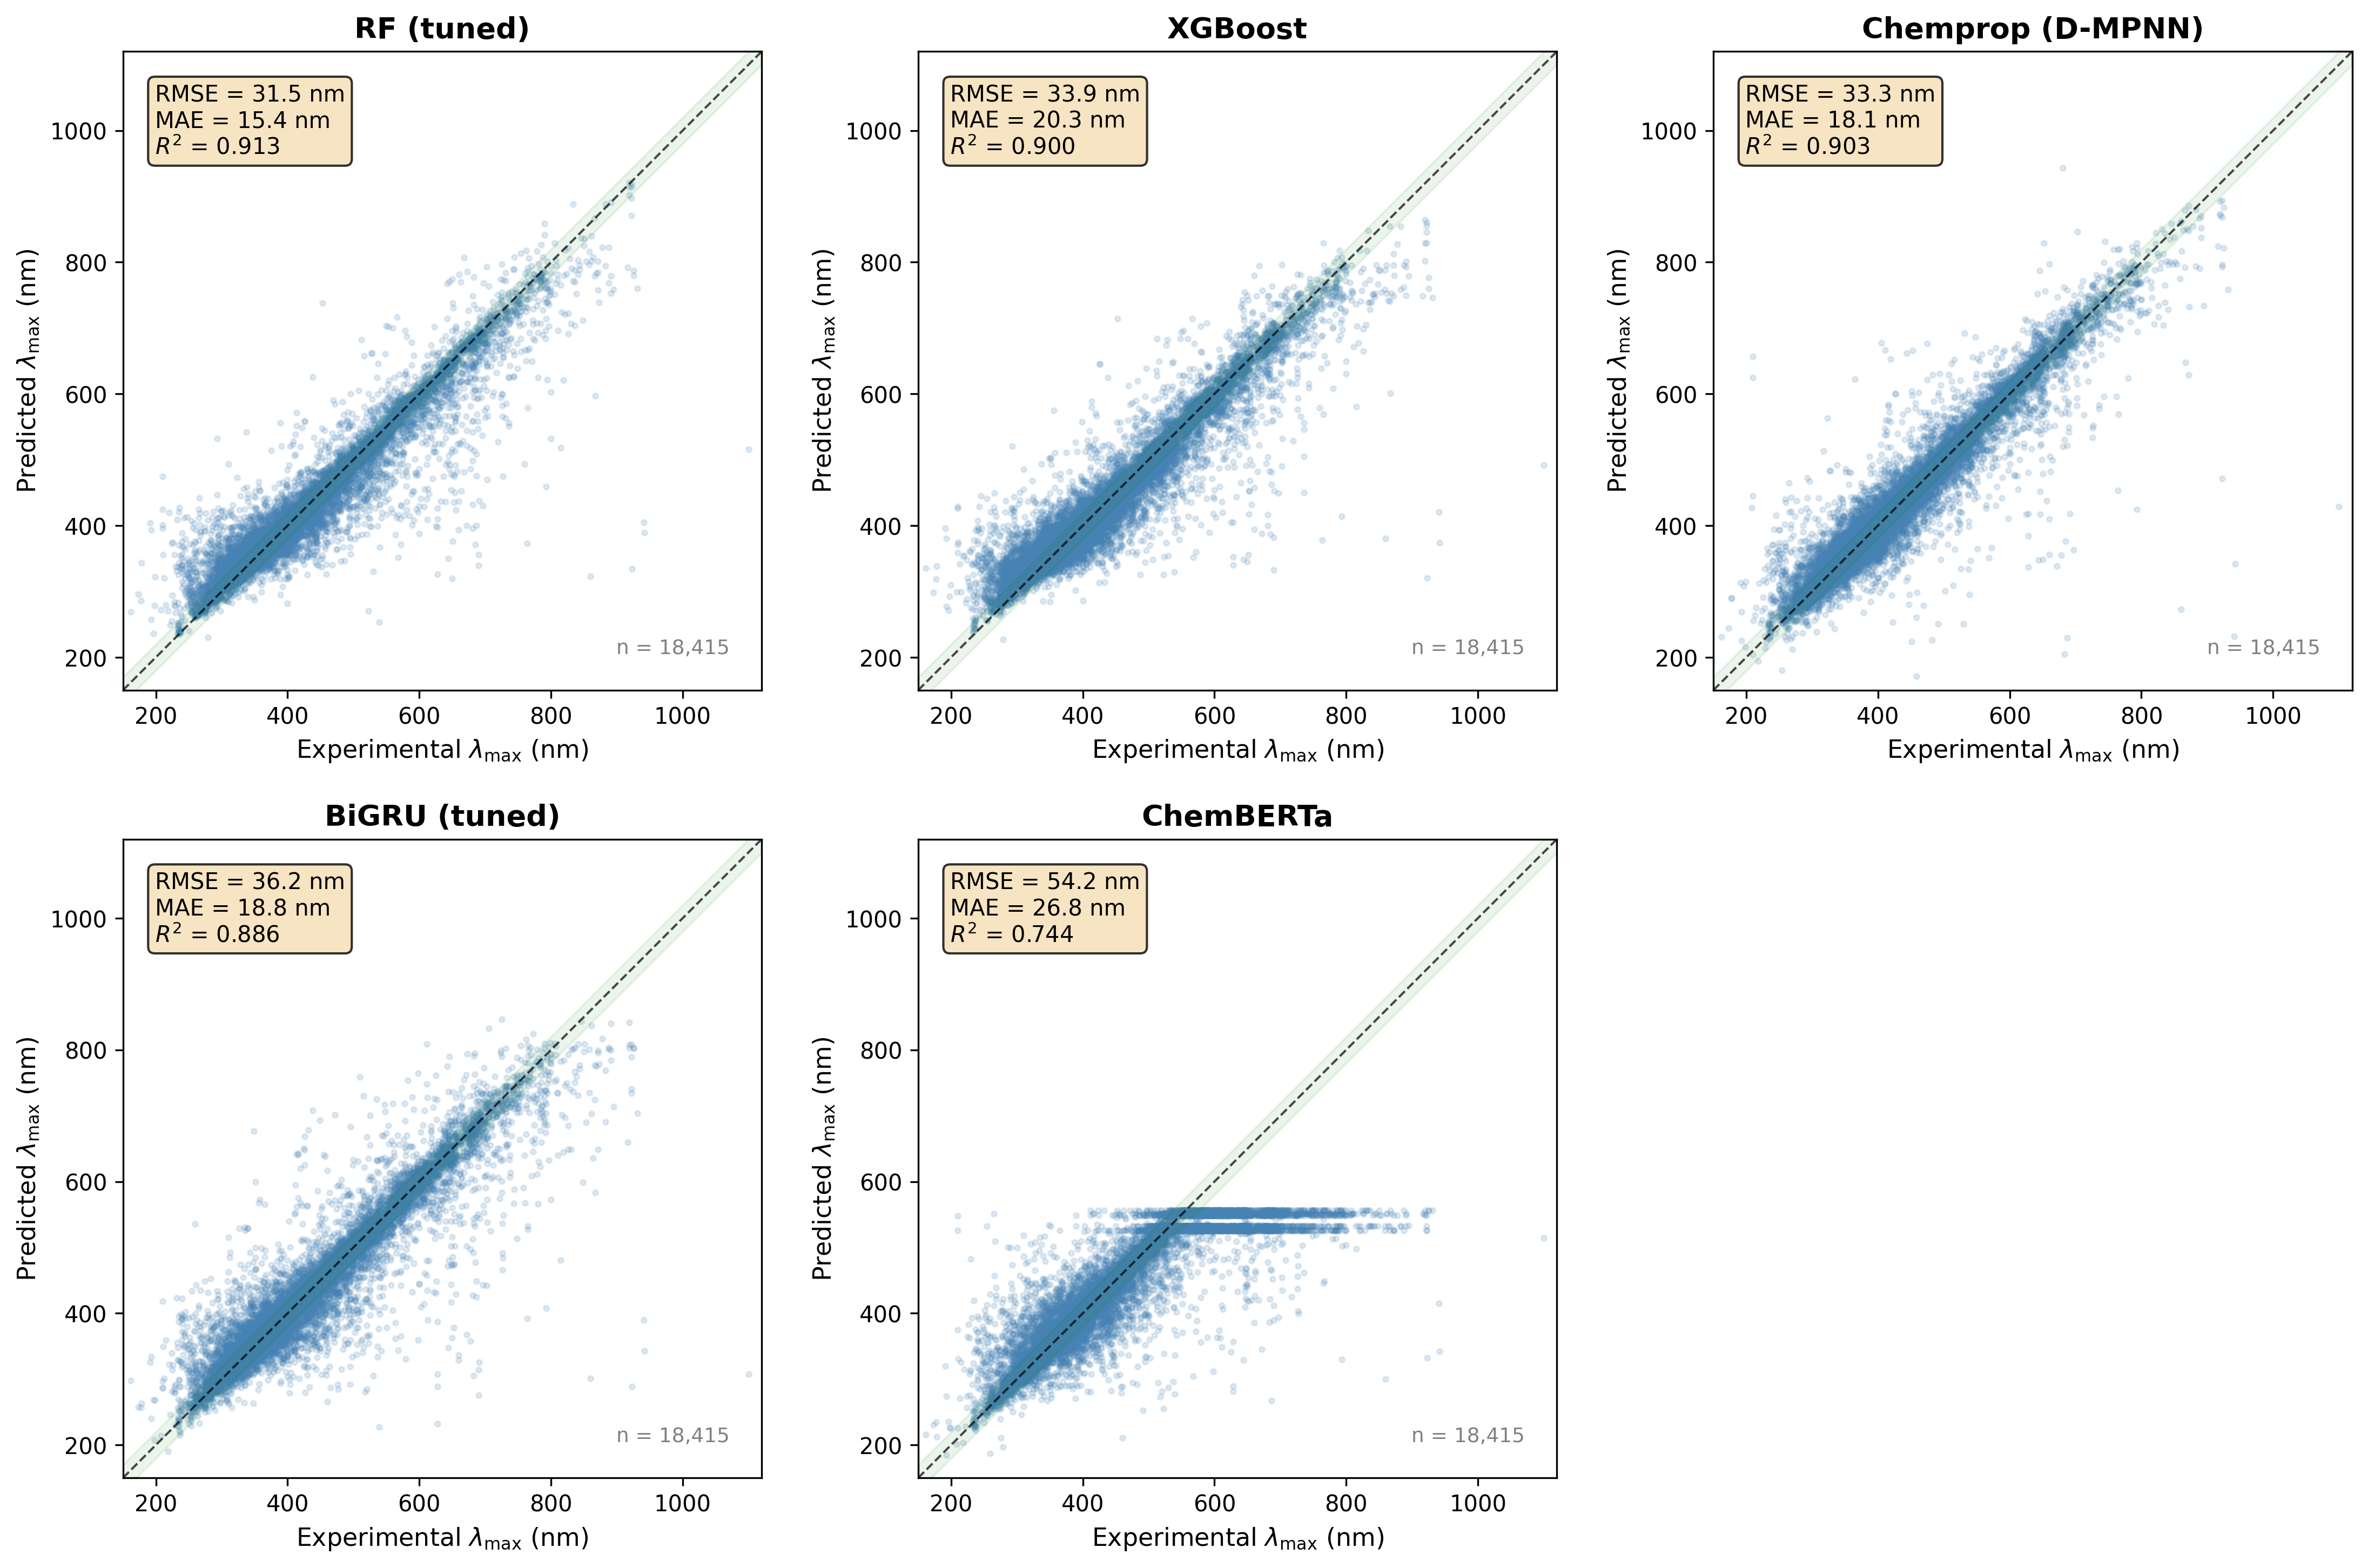
\includegraphics[width=0.95\textwidth]{results/parity_plot_5models.png}
    \caption{Parity plots for all five model families (pooled 5-fold CV predictions). Green bands: $\pm 20$~nm. RF and Chemprop show the tightest clustering; ChemBERTa shows the most scatter. All models show increased error for $\lambda_{\max} > 500$~nm.}
    \label{fig:parity_5models}
\end{figure*}

\begin{figure}[htbp]
    \centering
    \begin{subfigure}[t]{\columnwidth}
        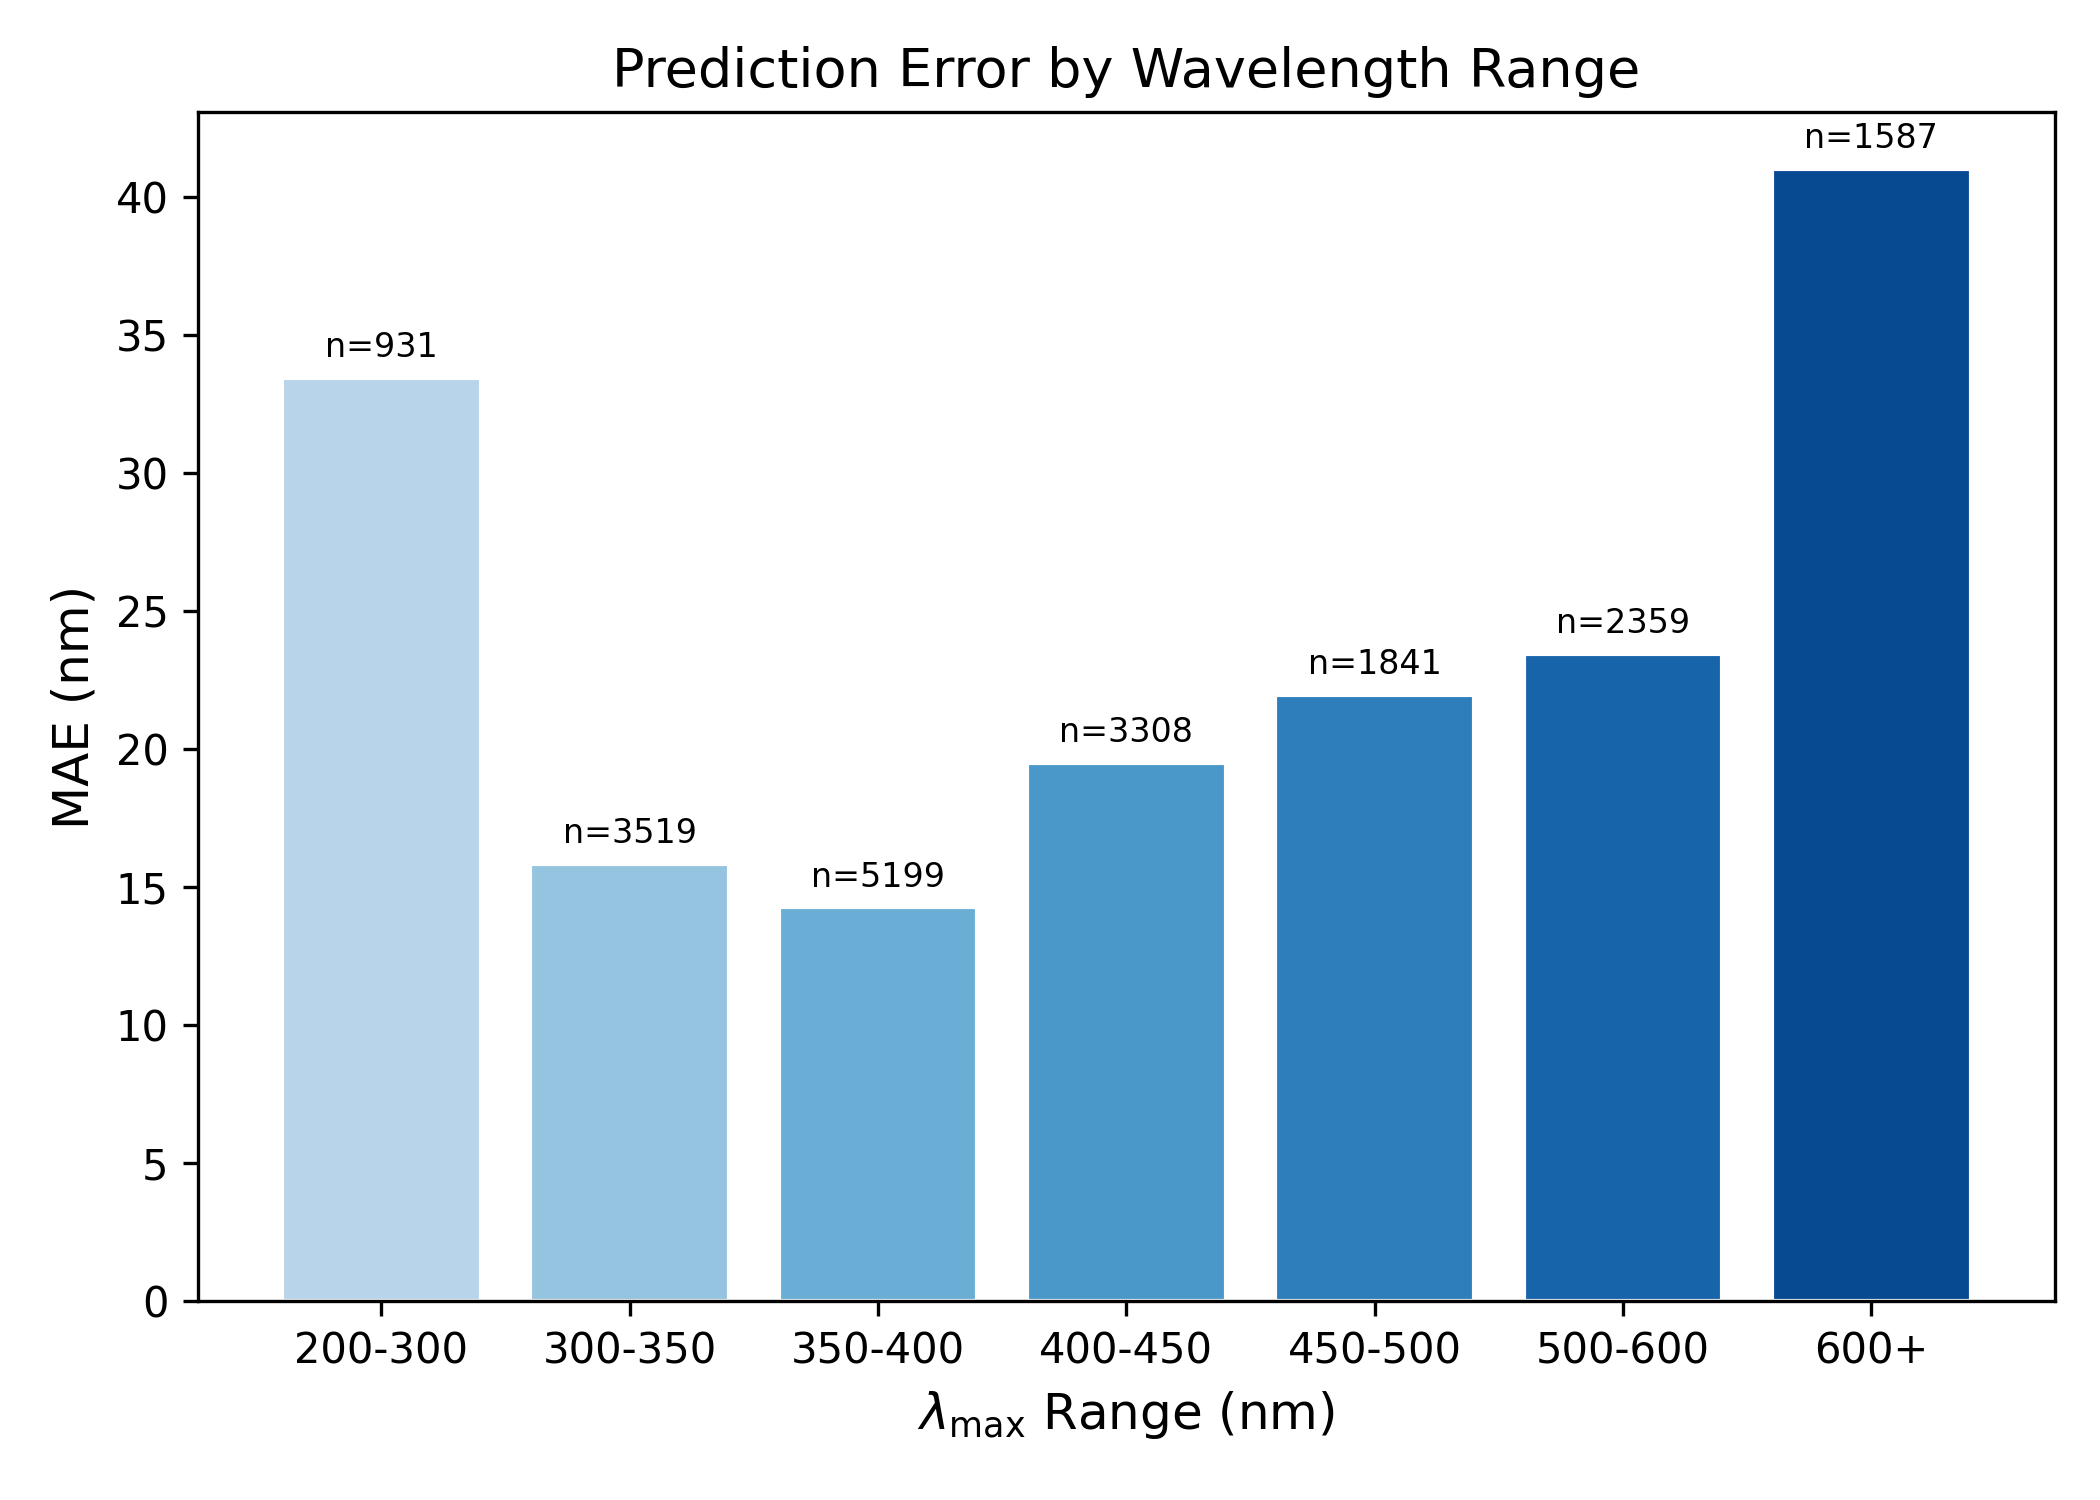
\includegraphics[width=\textwidth]{results/error_by_wavelength.png}
        \caption{MAE by wavelength range.}
    \end{subfigure}
    \begin{subfigure}[t]{\columnwidth}
        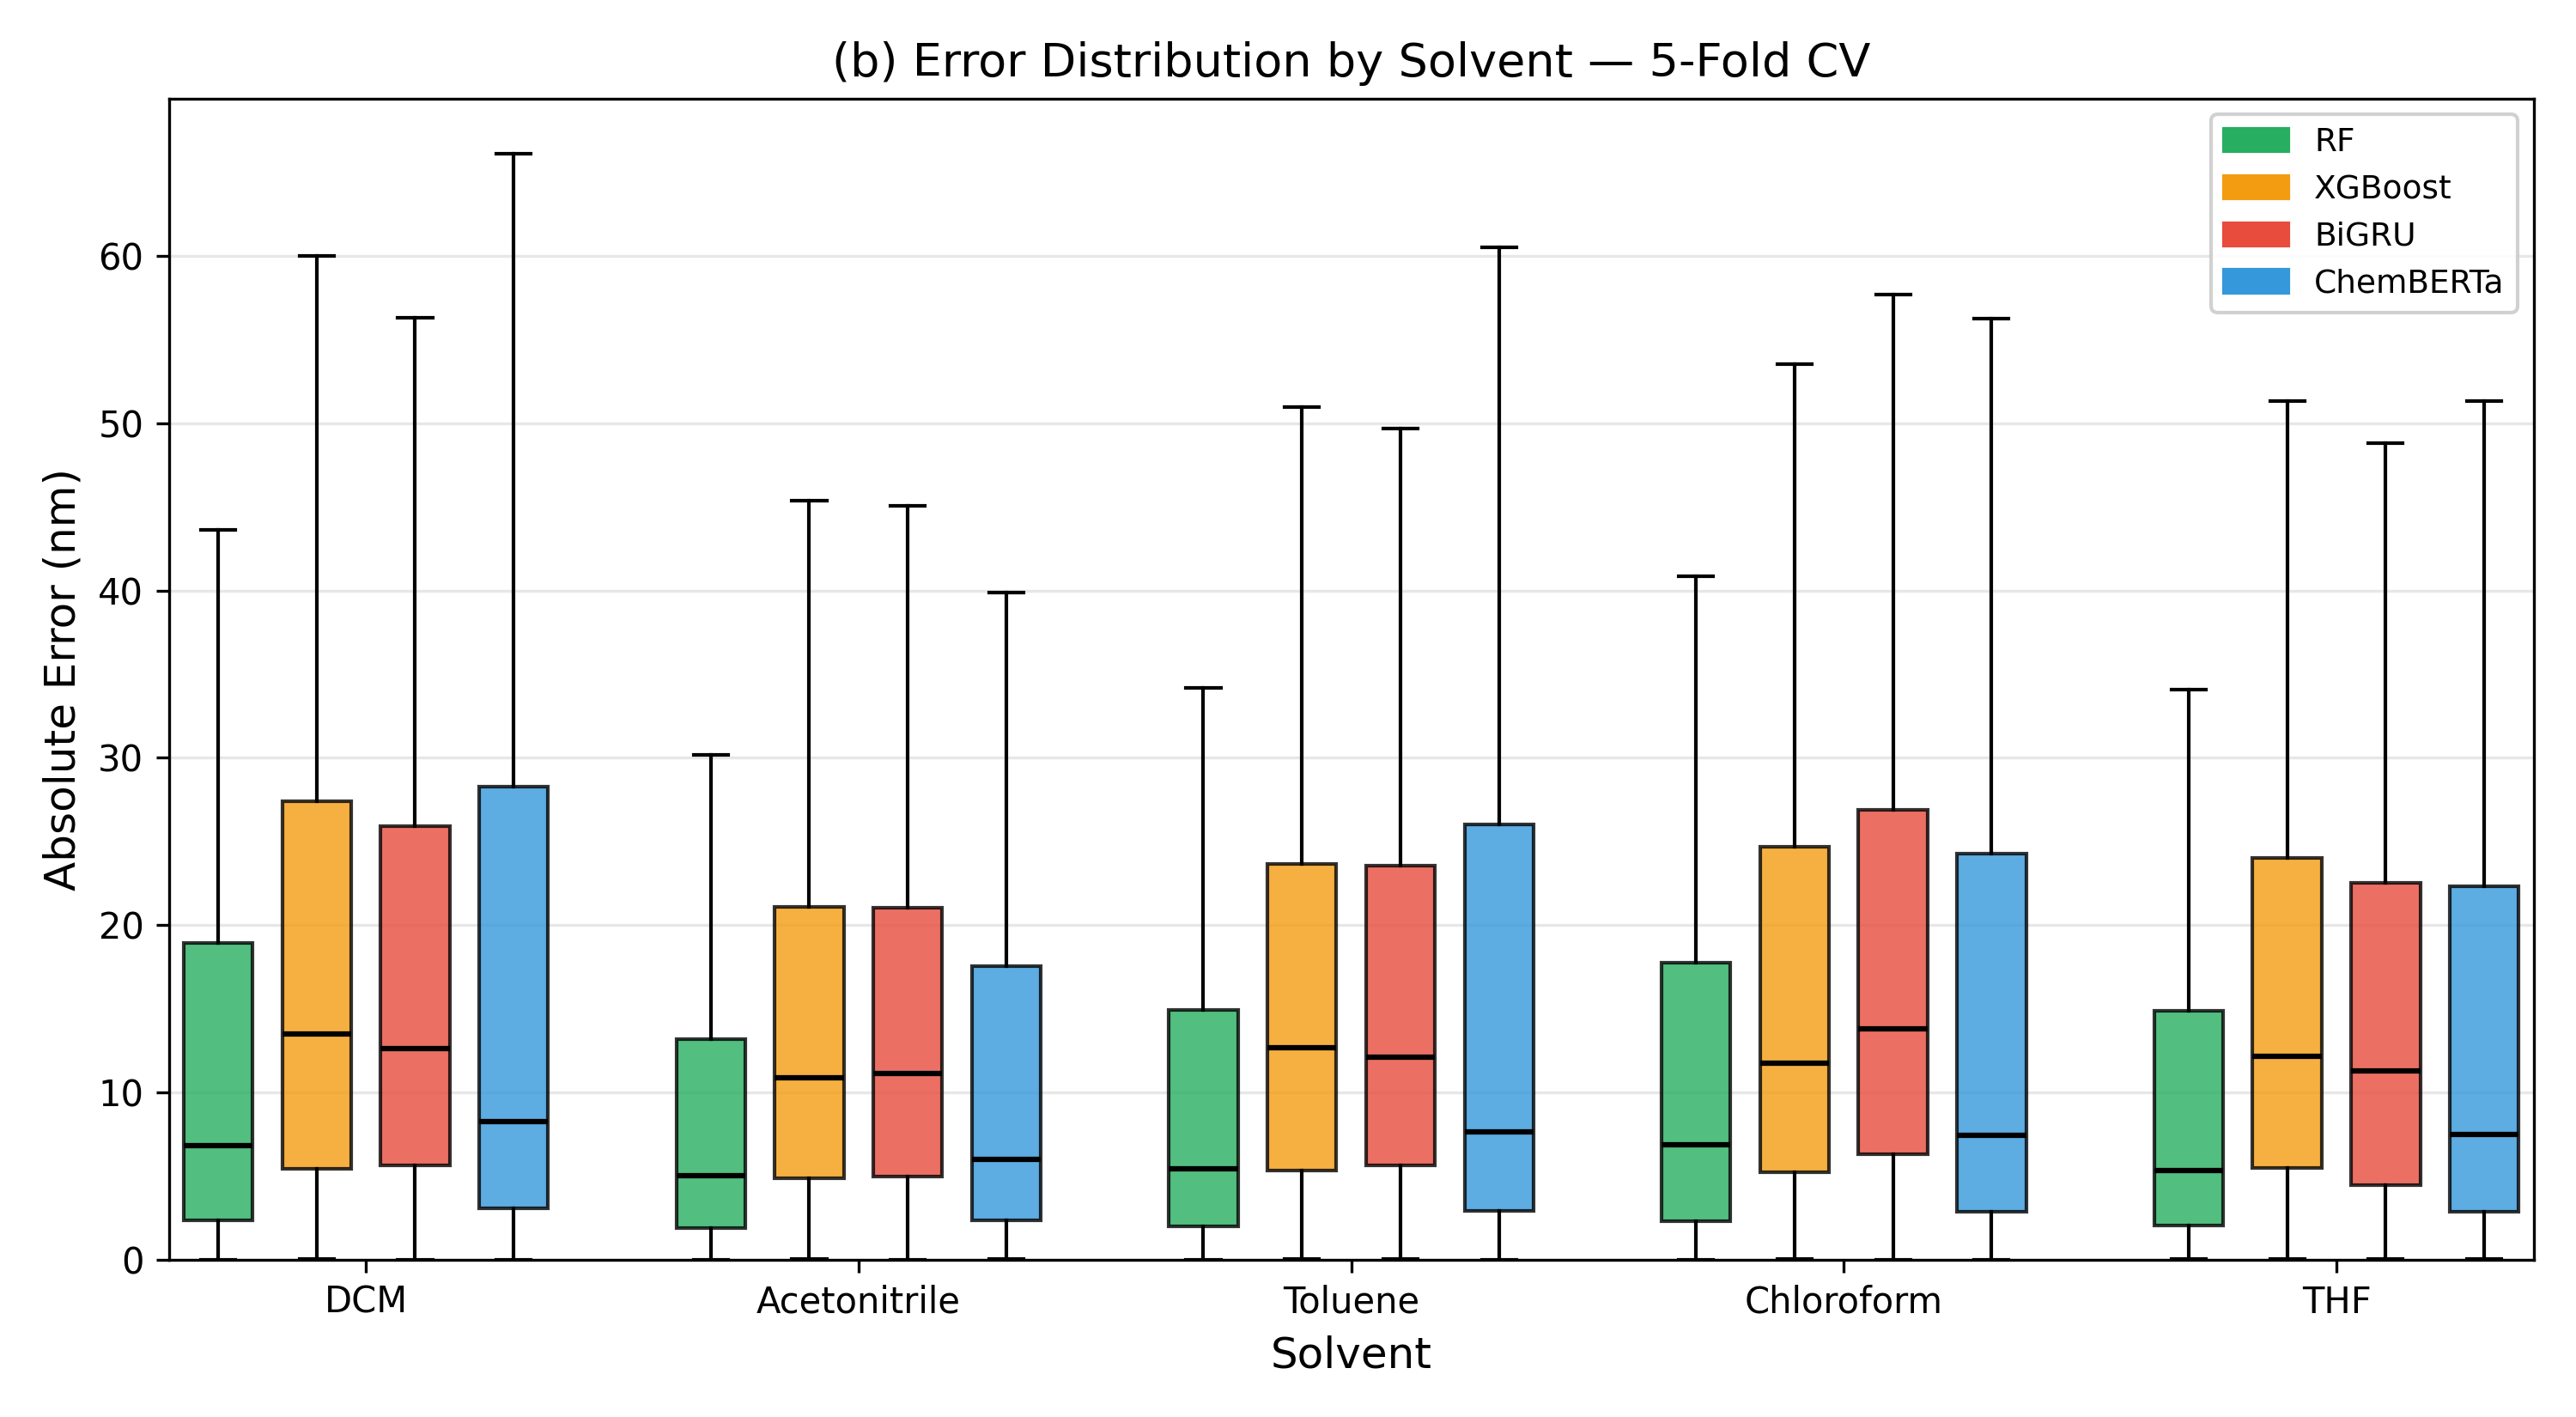
\includegraphics[width=\textwidth]{results/error_by_solvent.png}
        \caption{MAE by solvent type.}
    \end{subfigure}
    \caption{Error breakdown by wavelength range and solvent type for all five model families (pooled 5-fold CV).}
    \label{fig:error_breakdown}
\end{figure}

Figure~\ref{fig:parity_5models} shows parity plots for all five model families.
All models perform best in the 250--400~nm range where training data is most abundant (Figure~\ref{fig:error_breakdown}a).
Errors increase substantially for $\lambda_{\max} > 500$~nm, reflecting both data scarcity and the greater structural complexity of long-wavelength chromophores.\cite{flemingMolecular2010}
Error distributions across solvents (Figure~\ref{fig:error_breakdown}b) show relatively consistent performance, with slightly higher errors for chloroform and dichloromethane.

% Locality figure — wide
\begin{figure*}[!ht]
    \centering
    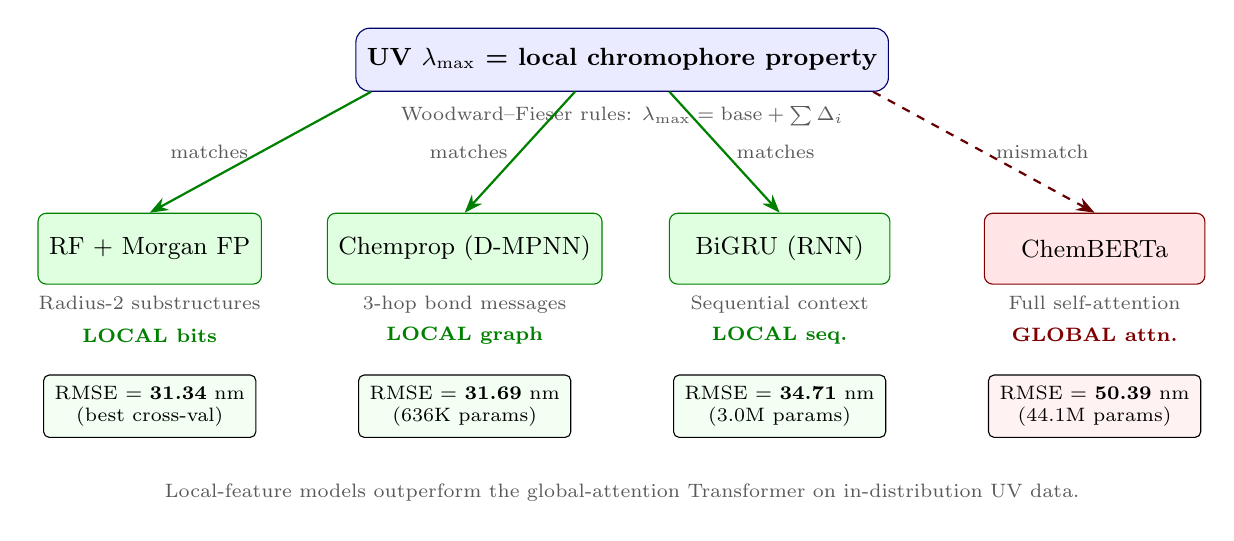
\begin{tikzpicture}[
        >=Stealth,
        box/.style={draw, rounded corners=3pt, minimum width=2.8cm, minimum height=0.9cm, align=center, font=\small},
        localbox/.style={box, fill=green!12, draw=green!50!black},
        globalbox/.style={box, fill=red!10, draw=red!50!black},
        propbox/.style={draw, rounded corners=5pt, fill=blue!8, draw=blue!40!black, minimum width=4cm, minimum height=0.8cm, align=center, font=\small\bfseries},
        annot/.style={font=\scriptsize, text=gray!70!black},
        every node/.style={inner sep=4pt}
    ]
    \node[propbox] (uvprop) at (0, 4.2) {UV $\lambda_{\max}$ = local chromophore property};
    \node[annot, below=1pt of uvprop] {Woodward--Fieser rules: $\lambda_{\max} = \text{base} + \sum \Delta_i$};
    \node[localbox] (rf) at (-6.0, 1.8) {RF + Morgan FP};
    \node[annot, below=0pt of rf] {Radius-2 substructures};
    \node[font=\scriptsize\bfseries, text=green!50!black] at (-6.0, 0.7) {LOCAL bits};
    \node[localbox] (chemprop) at (-2.0, 1.8) {Chemprop (D-MPNN)};
    \node[annot, below=0pt of chemprop] {3-hop bond messages};
    \node[font=\scriptsize\bfseries, text=green!50!black] at (-2.0, 0.7) {LOCAL graph};
    \node[localbox] (bigru) at (2.0, 1.8) {BiGRU (RNN)};
    \node[annot, below=0pt of bigru] {Sequential context};
    \node[font=\scriptsize\bfseries, text=green!50!black] at (2.0, 0.7) {LOCAL seq.};
    \node[globalbox] (bert) at (6.0, 1.8) {ChemBERTa};
    \node[annot, below=0pt of bert] {Full self-attention};
    \node[font=\scriptsize\bfseries, text=red!50!black] at (6.0, 0.7) {GLOBAL attn.};
    \draw[->, thick, green!50!black] (uvprop.south west) ++(0.2,0) -- (rf.north) node[midway, left, annot] {matches};
    \draw[->, thick, green!50!black] (uvprop.south) ++(-0.6,0) -- (chemprop.north) node[midway, left, annot] {matches};
    \draw[->, thick, green!50!black] (uvprop.south) ++(0.6,0) -- (bigru.north) node[midway, right, annot] {matches};
    \draw[->, thick, red!40!black, dashed] (uvprop.south east) ++(-0.2,0) -- (bert.north) node[midway, right, annot] {mismatch};
    \node[draw, rounded corners=2pt, fill=green!5, font=\scriptsize, align=center] at (-6.0, -0.2) {RMSE = \textbf{31.34} nm\\(best cross-val)};
    \node[draw, rounded corners=2pt, fill=green!5, font=\scriptsize, align=center] at (-2.0, -0.2) {RMSE = \textbf{31.69} nm\\(636K params)};
    \node[draw, rounded corners=2pt, fill=green!5, font=\scriptsize, align=center] at (2.0, -0.2) {RMSE = \textbf{34.71} nm\\(3.0M params)};
    \node[draw, rounded corners=2pt, fill=red!5, font=\scriptsize, align=center] at (6.0, -0.2) {RMSE = \textbf{50.39} nm\\(44.1M params)};
    \node[annot, text width=12cm, align=center] at (0, -1.3) {Local-feature models outperform the global-attention Transformer on in-distribution UV data.};
    \end{tikzpicture}
    \caption{Locality-of-property hypothesis. UV $\lambda_{\max}$ is determined by local chromophore features, favoring models whose inductive bias encodes local molecular neighborhoods.}
    \label{fig:local_vs_global}
\end{figure*}


\subsection{Model Interpretability}
\label{sec:interpretability}

A key advantage of fingerprint-based models is their interpretability.
RF models provide direct access to each feature's contribution through Gini importance, a measure of how much each feature reduces prediction variance across all trees.
Since each Morgan fingerprint bit corresponds to a specific molecular substructure, high-importance bits can be decoded back to chemically meaningful motifs.

\begin{figure}[htbp]
    \centering
    \begin{subfigure}[t]{\columnwidth}
        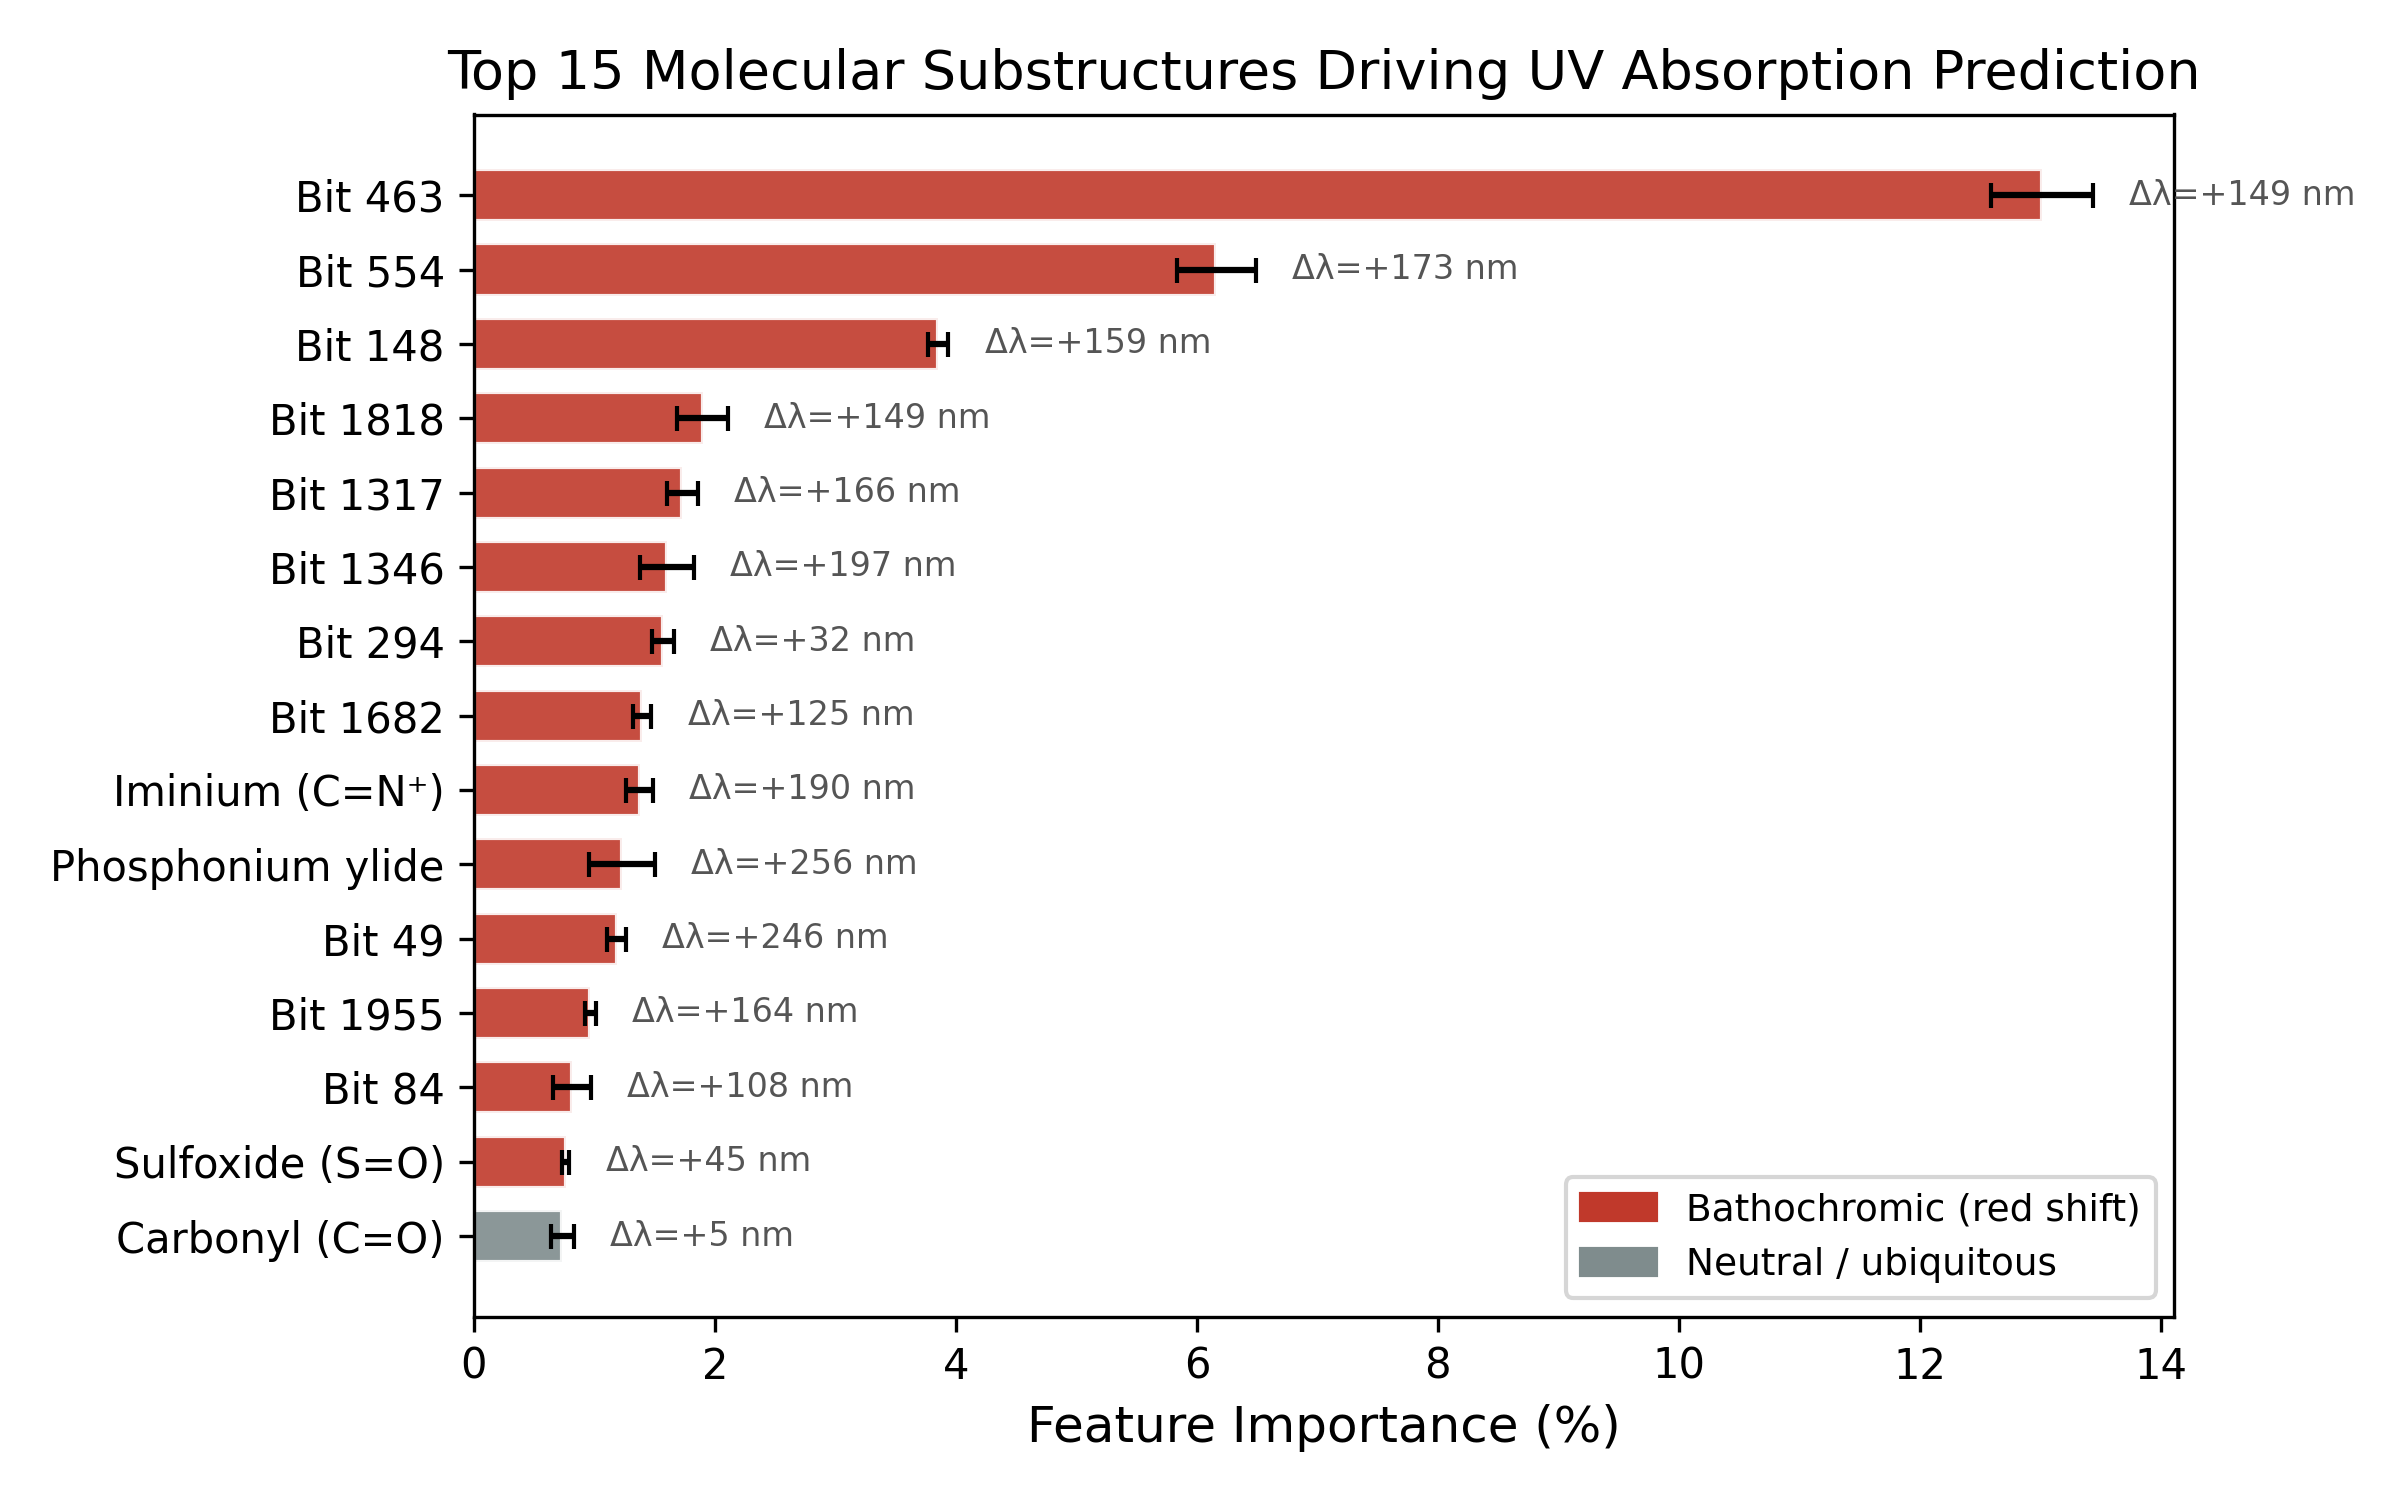
\includegraphics[width=\textwidth]{results/rf_feature_importance.png}
        \caption{Top 15 Morgan fingerprint bits ranked by Gini importance. Red indicates bathochromic (red-shifting) substructures; gray indicates neutral or ubiquitous features.}
    \end{subfigure}
    \begin{subfigure}[t]{\columnwidth}
        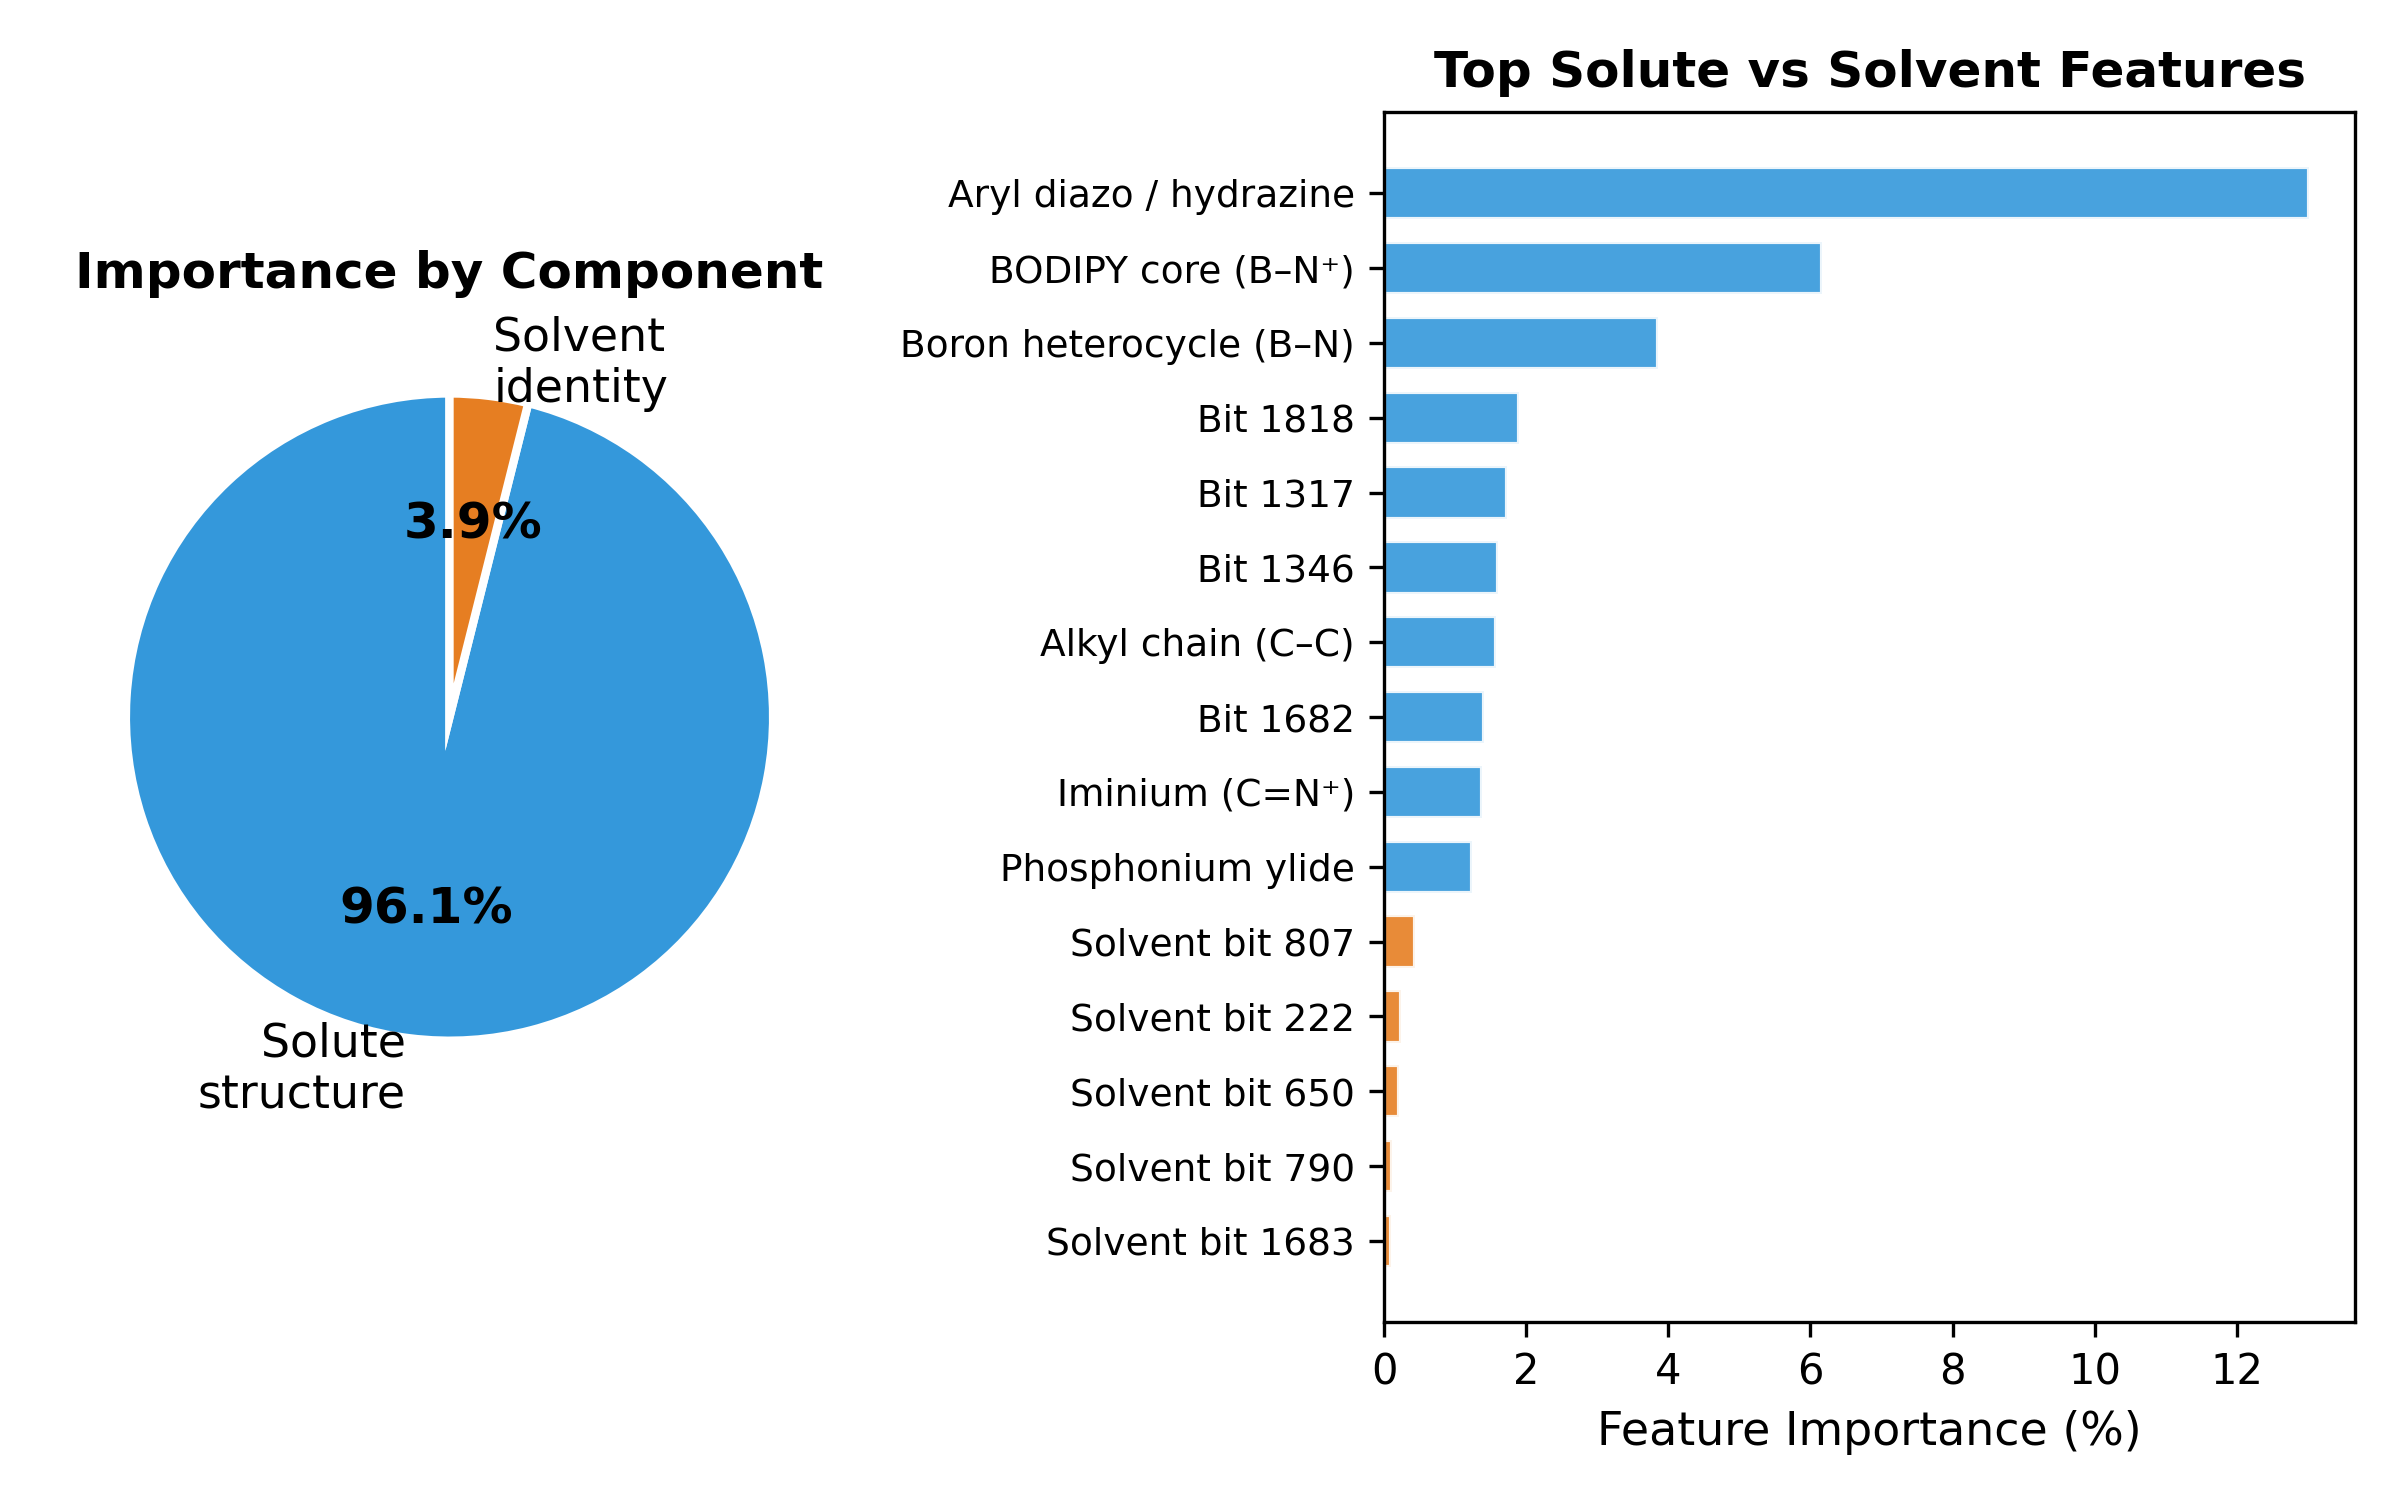
\includegraphics[width=\textwidth]{results/rf_solute_vs_solvent.png}
        \caption{Solute vs.\ solvent fingerprint importance.}
    \end{subfigure}
    \caption{RF feature importance analysis. The model learns chemically meaningful patterns: top features correspond to known chromophore motifs.}
    \label{fig:rf_interpretability}
\end{figure}

The most important feature (bit 463, 12.7\% importance) corresponds to aryl diazo/hydrazine substructures ($\Delta\lambda_{\max} = +143$~nm).
Solute structure accounts for 96.1\% of total importance (Figure~\ref{fig:rf_interpretability}b).

\begin{figure}[htbp]
    \centering
    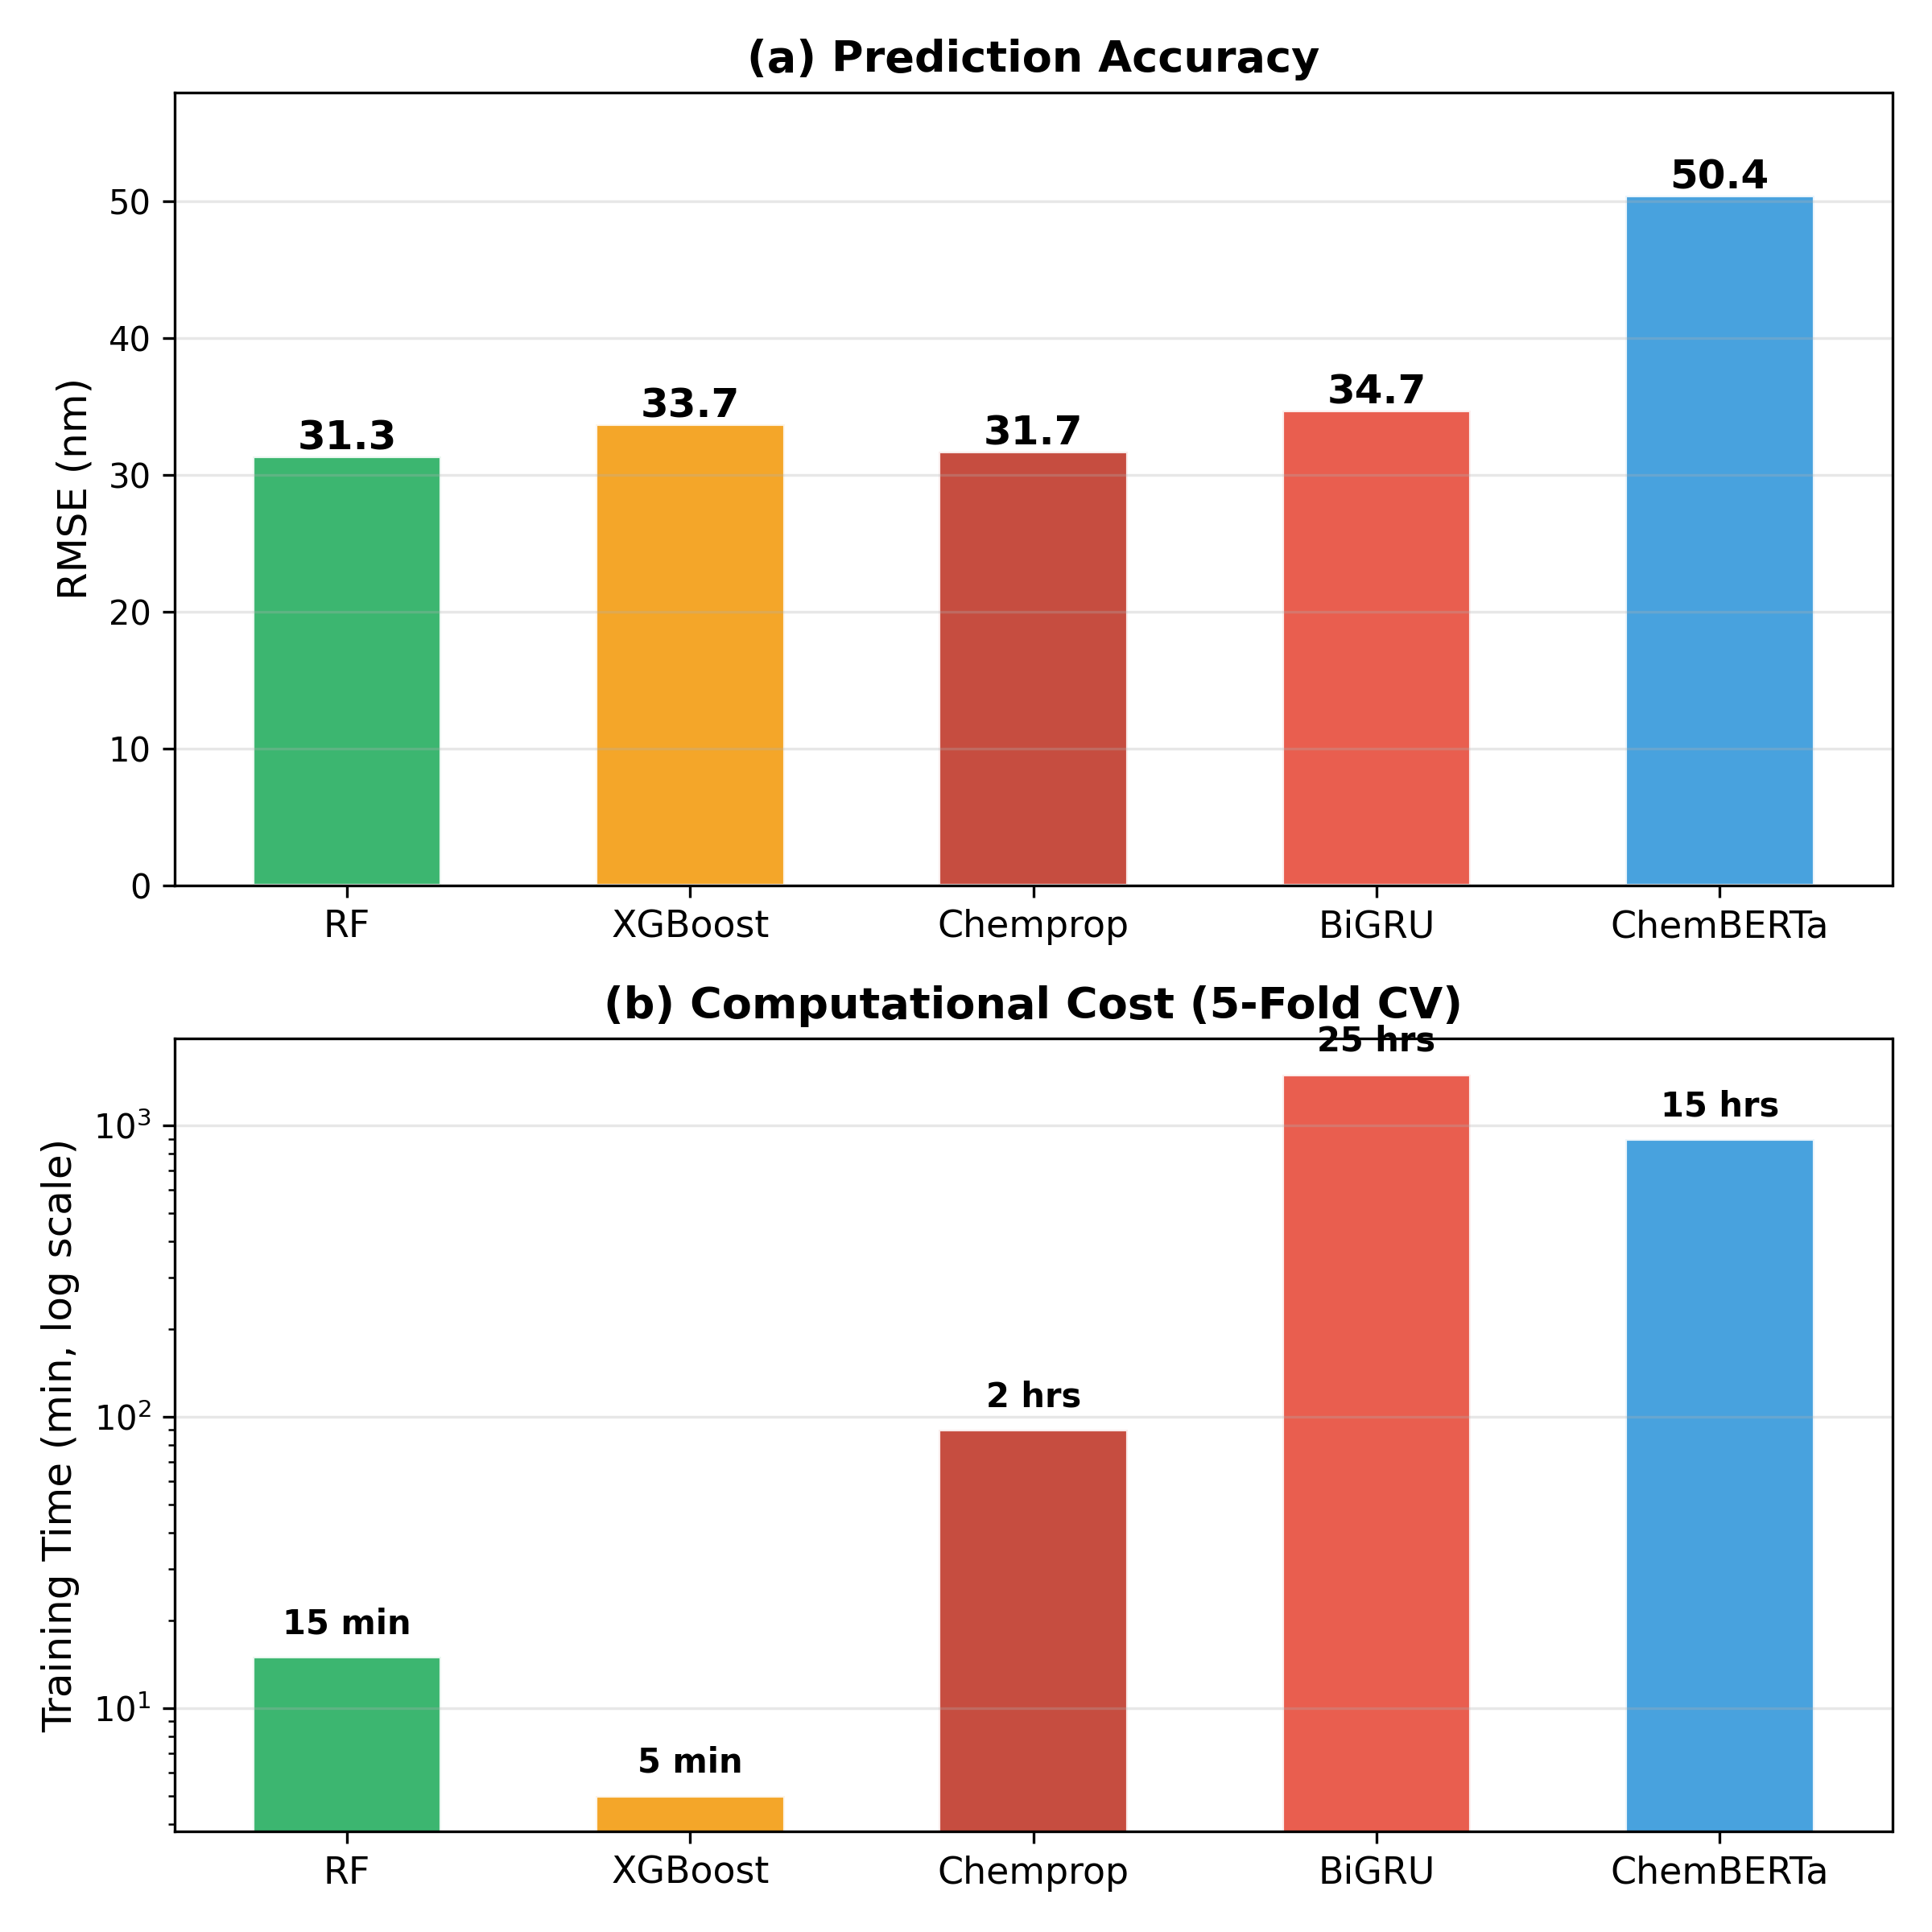
\includegraphics[width=\columnwidth]{results/rf_training_comparison.png}
    \caption{Training time vs.\ performance. RF achieves the best RMSE in 15~min on CPU; Chemprop requires 1.5~h and BiGRU 25~h on GPU.}
    \label{fig:rf_practical}
\end{figure}

\textbf{Practical advantages.}
RF training completes in approximately 15 minutes on a single CPU, compared to 1.5 hours for Chemprop and 25 hours for BiGRU on GPU, while achieving comparable or lower RMSE (Figure~\ref{fig:rf_practical}).

\textbf{BiGRU gradient saliency.}
We computed Input$\times$Gradient saliency\cite{simonyan2014deep} for each SMILES character position, mapped to atoms via RDKit,\cite{landrumRdkitRdkit2020_03_12020} and visualized as 2D heatmaps (Figure~\ref{fig:bigru_saliency}).
High-saliency atoms concentrate on heteroatoms (O, N, S) and atoms adjacent to double bonds, consistent with RF feature importance.

% Saliency — wide figure
\begin{figure*}[!ht]
    \centering
    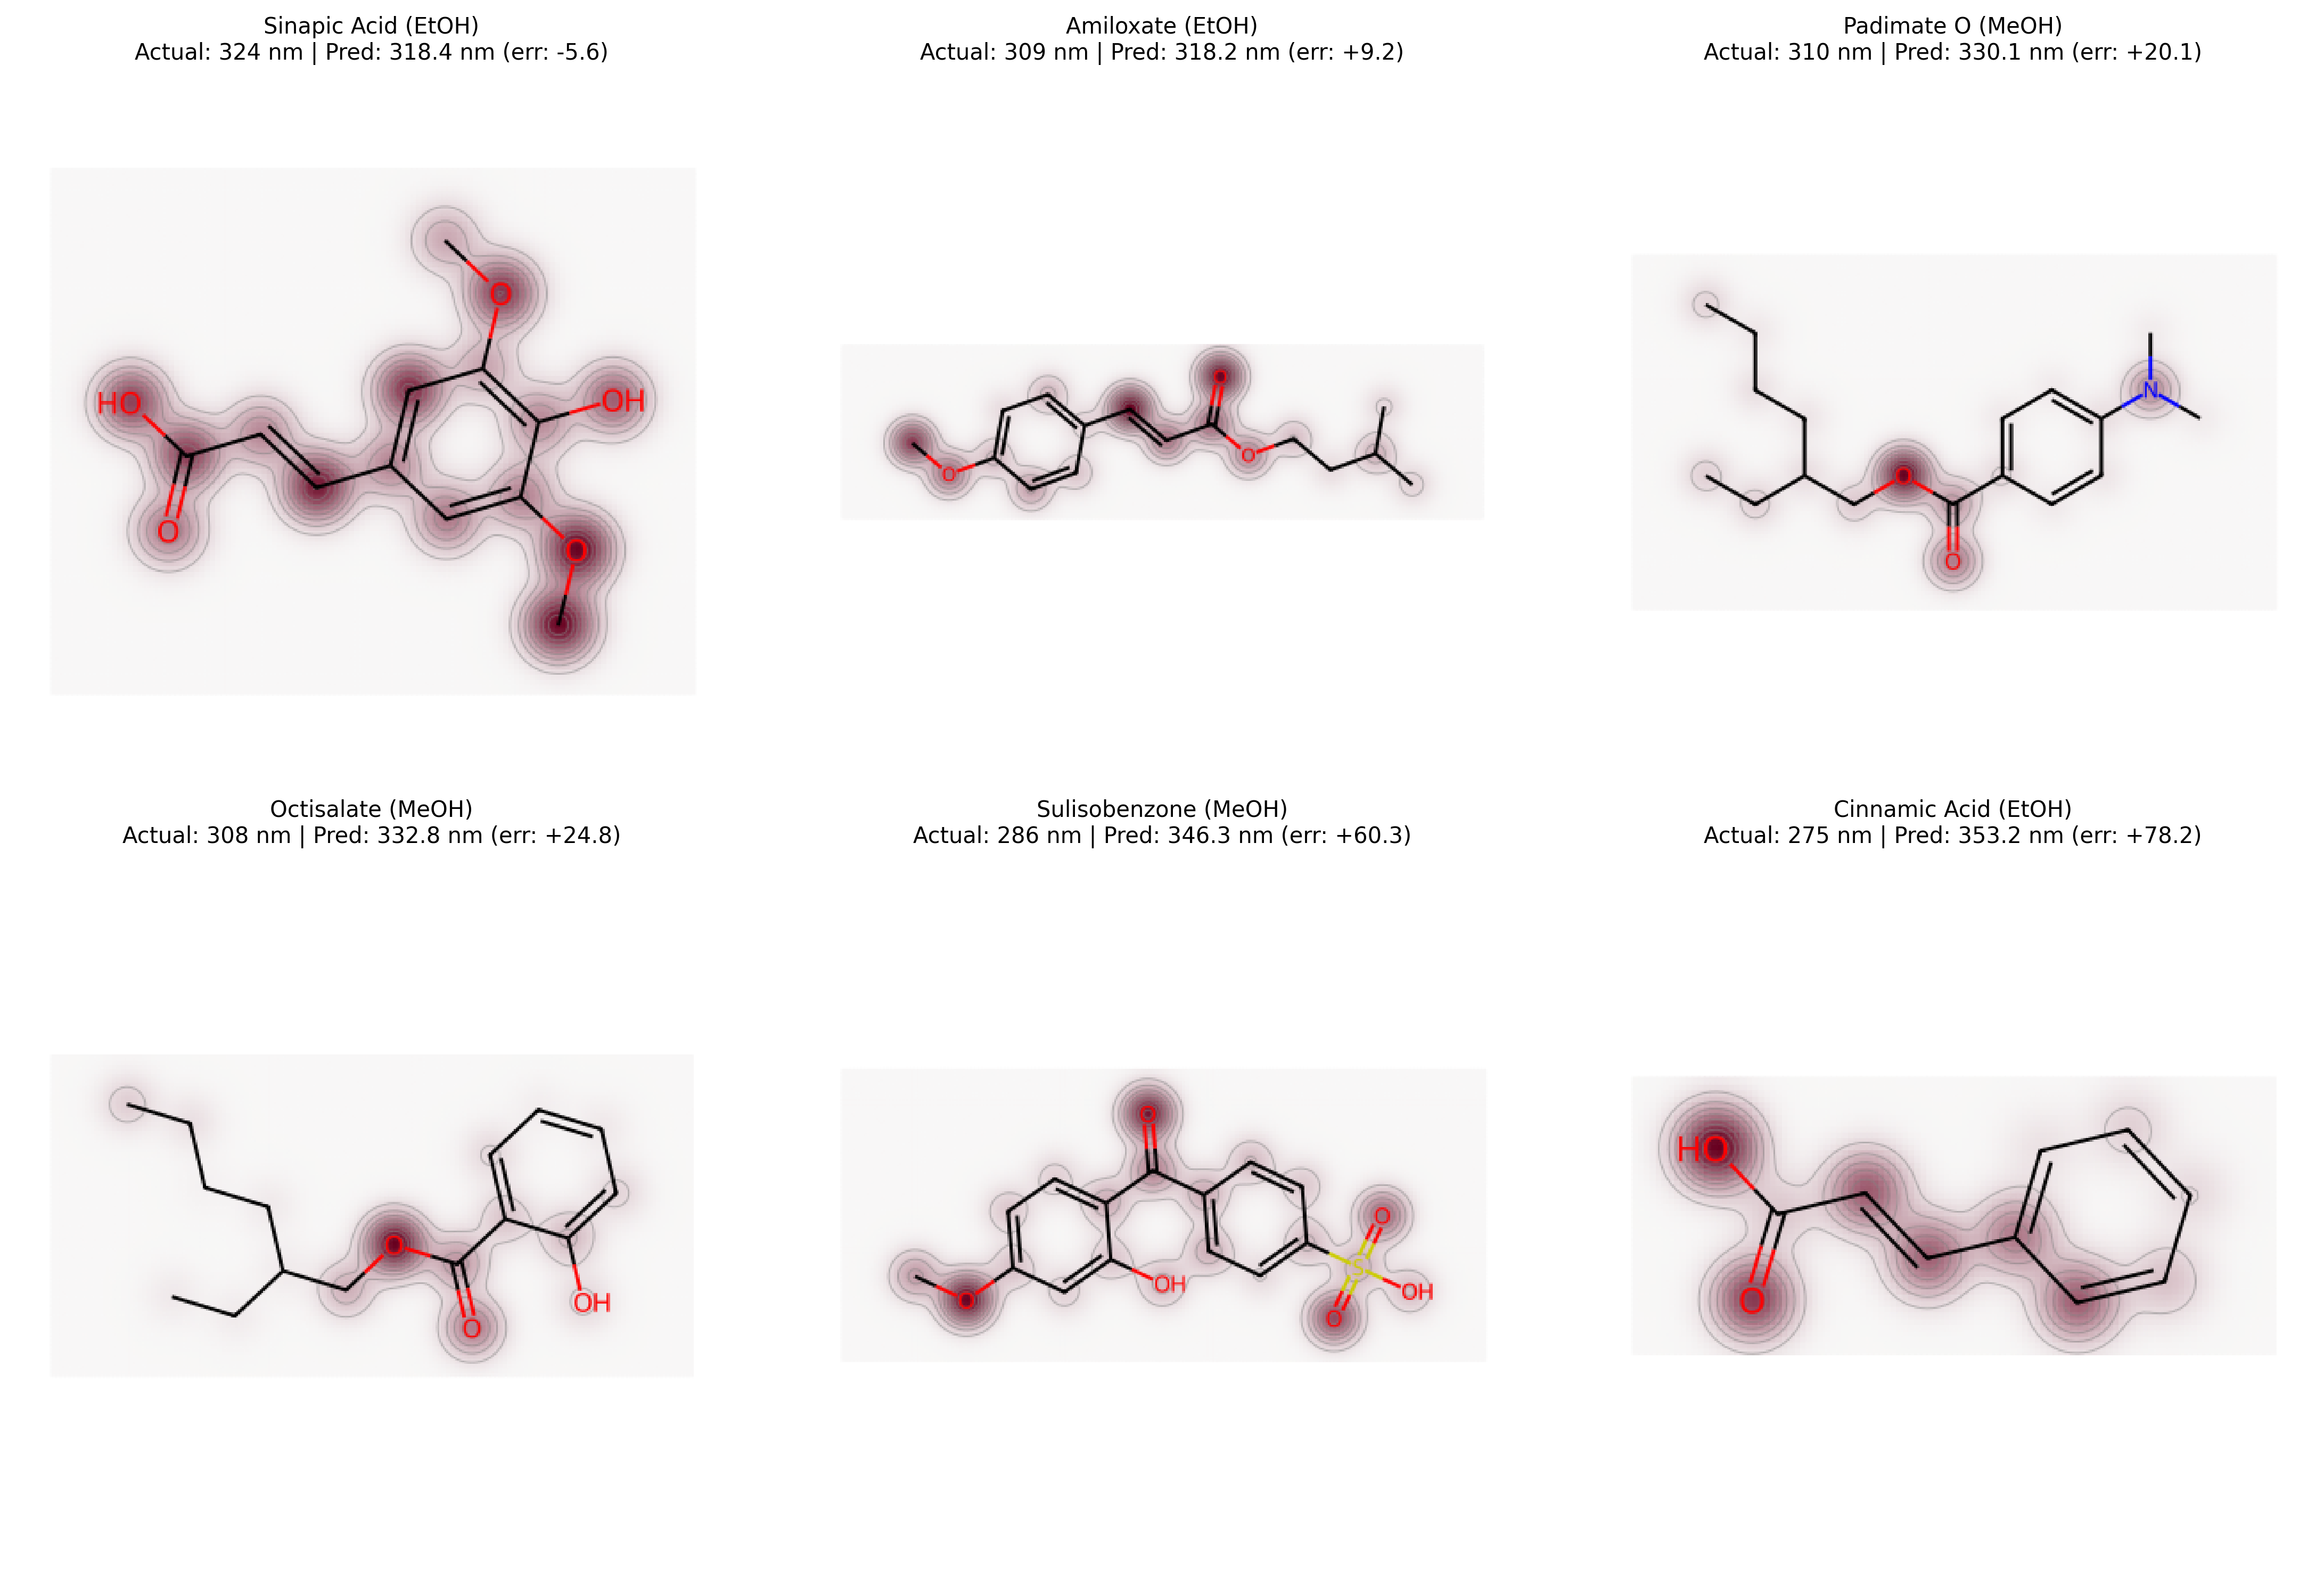
\includegraphics[width=0.95\textwidth]{results/bigru_saliency_atoms.png}
    \caption{BiGRU gradient saliency mapped to 2D molecular structures for six wetlab validation molecules. Atom color intensity reflects gradient-based importance (red = high saliency). Top row: well-predicted molecules; bottom row: poorly predicted molecules. Overlap with RF feature importance confirms both architectures learn meaningful photochemistry.}
    \label{fig:bigru_saliency}
\end{figure*}


\subsection{Photosafety Classification}
\label{sec:classification}

We apply our models to ICH~S10\cite{ICH2013S10} photosafety classification using the Mamede et al.\cite{mamede2021machine} protocol.

\begin{table}[htbp]
\centering
\caption{Photosafety classification. $^\dagger$Published result.}
\label{tab:classification}
\small
\begin{tabular}{lcccc}
\toprule
\textbf{Model} & \textbf{Sens.} & \textbf{Spec.} & \textbf{Acc.} & \textbf{AUC} \\
\midrule
Mamede RF$^\dagger$ & 0.90  & 0.88  & 0.89  & --- \\
Our RF              & 0.876 & 0.882 & 0.879 & 0.942 \\
BiGRU cls           & 0.794 & 0.811 & 0.803 & 0.886 \\
\bottomrule
\end{tabular}
\end{table}

Our RF classifier closely reproduces published results (accuracy 0.879 vs.\ 0.89), validating the effectiveness of Morgan fingerprints for photosafety screening.


\subsection{Experimental Validation}
\label{sec:experimental}

We measured UV absorption spectra for 16 commercially available compounds in both ethanol and methanol, yielding 32 experimental $\lambda_{\max}$ values.
Of these 16 molecules, 15 are entirely absent from the training dataset.

\begin{table}[htbp]
\centering
\caption{Aggregate wetlab validation (16 molecules $\times$ 2 solvents = 32 points). 95\% bootstrap CIs.}
\label{tab:wetlab_summary}
\small
\begin{tabular}{lcc}
\toprule
\textbf{Model} & \textbf{MAE [95\% CI]} & \textbf{RMSE [95\% CI]} \\
\midrule
Chemprop     & \textbf{26.2}              & 35.7 \\
ChemBERTa    & 26.3 [20.1--33.0] & \textbf{32.2} [25.2--38.8] \\
BiGRU (def.) & 28.6 [22.7--35.0] & 33.9 [26.2--41.2] \\
BiGRU (tuned)& 31.5              & 37.0 \\
RF           & 38.5 [31.6--45.9] & 43.7 [35.3--51.7] \\
\bottomrule
\end{tabular}
\end{table}

On novel compounds, all deep learning models (Chemprop MAE = 26.2~nm, ChemBERTa 26.3~nm, BiGRU 28.6~nm) outperform RF (38.5~nm), demonstrating that learned representations generalize where fixed fingerprints cannot.
RF's advantage on cross-validated benchmarks reverses on out-of-distribution data, highlighting the complementary strengths of classical and deep learning approaches.

\begin{figure}[htbp]
    \centering
    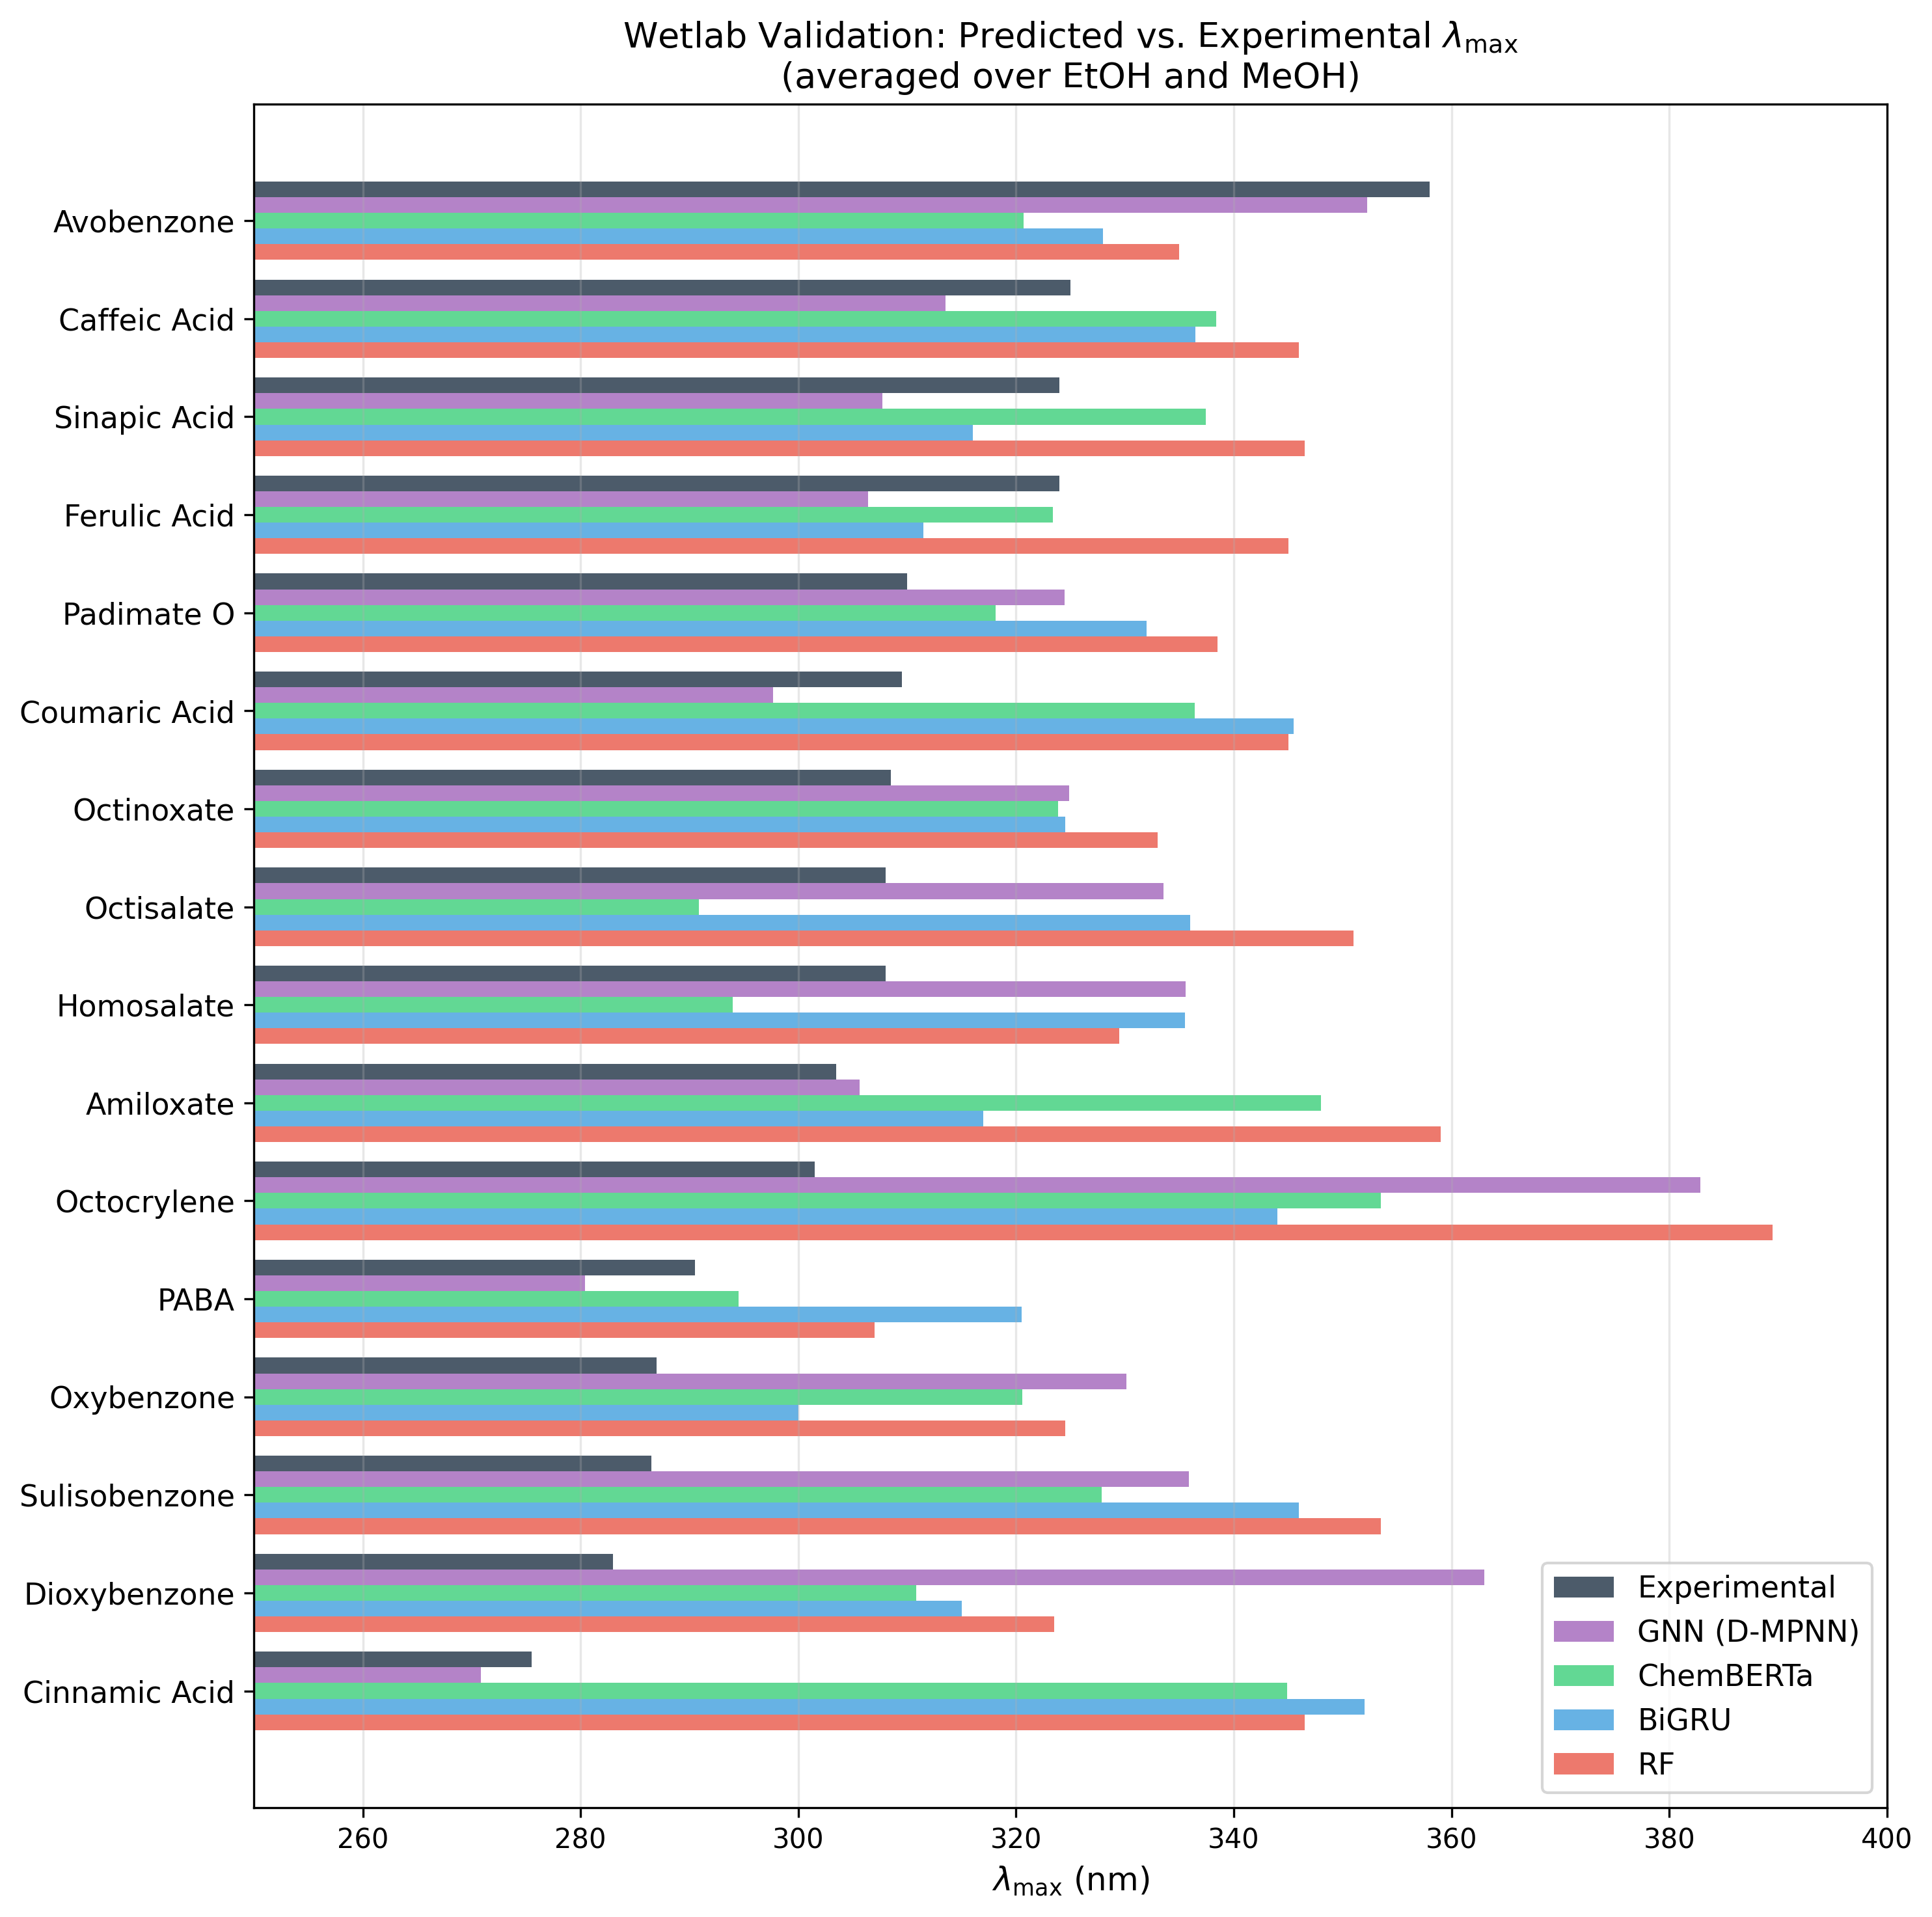
\includegraphics[width=\columnwidth]{results/wetlab_per_molecule.png}
    \caption{Per-molecule comparison of experimental and predicted $\lambda_{\max}$ for 16 sunscreen-related compounds, averaged over EtOH and MeOH.}
    \label{fig:wetlab_per_molecule}
\end{figure}


% ===== Conclusion =====
\section{Conclusion}
\label{sec:conclusion}

We have presented a systematic benchmark of ML approaches for UV absorption prediction, comparing RF, XGBoost, Chemprop (D-MPNN), BiGRU, and ChemBERTa across three datasets totaling over 60,000 molecules.
Our key findings are:

\begin{enumerate}
    \item \textbf{RF and deep learning have complementary strengths.}
    RF and Chemprop are statistically tied on cross-validation (RMSE = 31.34 vs.\ 31.69~nm, $p = 0.77$), both outperforming BiGRU and ChemBERTa. On novel compounds, all deep learning models outperform RF.

    \item \textbf{Solvent encoding helps all architectures.}
    A simple concatenation strategy reduces RMSE by 6--8\% across fingerprint, graph, and recurrent models (all $p < 0.02$).

    \item \textbf{Both model families offer interpretability.}
    RF provides global interpretability through feature importance; BiGRU provides instance-level interpretability through gradient saliency. Both highlight the same chromophore motifs.

    \item \textbf{Practical classification favors fingerprints.}
    RF-based photosafety classification (accuracy = 0.879) closely reproduces the published Mamede benchmark (0.89).
\end{enumerate}

More broadly, when a target property is determined by local molecular features, models with local inductive bias outperform global-attention architectures on in-distribution benchmarks, while pretrained Transformers retain advantages for out-of-distribution generalization.

\subsection*{Limitations}

Our models use 1D or 2D representations; 3D conformational information may matter for structurally diverse chromophores.\cite{lupopasini2023excited}
The experimental validation set (16 molecules) is small.
ChemBERTa hyperparameters remain untuned due to prohibitive training cost.
The tuned BiGRU shows \textit{worse} OOD performance (MAE = 31.5~nm) than the default (28.6~nm), suggesting overfitting to in-distribution patterns.

\subsection*{Future Work}

Transfer learning from larger UV databases may improve deep learning performance.\cite{vermeire2021transfer}
Incorporating 3D structural information\cite{lupopasini2023excited} could improve predictions for geometry-dependent chromophores.
Ensemble approaches combining RF and deep learning could exploit complementary strengths.
Extending this benchmarking framework to emission wavelength, molar extinction coefficient, and lipophilicity will test whether the locality-of-property hypothesis generalizes.


% ===== Data and Code Availability =====
\section*{Data and Code Availability}
The primary Joung+Beard dataset and Deep4Chem database are available from Figshare\cite{joung2020experimental, beard2019comparative} (DOI: 10.6084/m9.figshare.12045567).
Additional dataset: Jung et al.\ (GitHub).\cite{jung2024machine}
All code will be released on GitHub under the MIT license upon publication.


\section*{Acknowledgments}
The authors thank the University of Iowa and the Midwest Bioprocessing Center for computational resources.
The authors declare no competing financial interest.

\section*{Supporting Information}
Per-fold cross-validation results (Tables~S1--S7), statistical significance tests (Table~S8), RF hyperparameter sensitivity, BiGRU and ChemBERTa learning curves (Figures~S1--S2), hyperparameter tuning asymmetry (Table~S9), and BiGRU character-type saliency (Figure~S3).


% ===== Bibliography =====
\bibliographystyle{achemso}
\bibliography{Proposal}

\end{document}
